
\chapter{走向仿射概形：底集合，与拓扑空间}
\label{ch:toward-affine-schemes}

\epigraph{格罗滕迪克如何想出概形的定义，这算不上一个严肃的历史问题——概形早已呼之欲出。塞尔说得好：概形并非任何人的发明……真正的问题在于：是什么让格罗滕迪克相信，他应当用这个定义，去把塞尔一篇 80 页的论文「化简」成上千页的《代数几何原理》（Éléments de Géométrie Algébrique）？}{——C.~\trMcLarty，[Mc, p.~313]}


我们现在已准备好来考虑\emph{\trScheme}的观念，它乃是\trAlgebraicGeometry{}中居于核心
地位的那一类几何空间。我们应当先把「几何空间」指的是什么想清楚。你多半已经见过
流形这一观念；我们希望将这个观念抽象化，使它能够推广到其他场合——尤其是使我们
得以处理非光滑的对象与算术的对象。


\section{走向概形}

从「\trManifold{}这类东西」的观念推广到更为万能的「\trGeometricSpace」观念，其背后的关键洞见如下：一个\trGeometricSpace{}（比如一个\trManifold{}）是可以通过理解其上的函数而被透彻理解的。更精确地说，我们将通过该空间上的函数\trSheaf{}来理解它。若你感兴趣的是\trDifferentiable\trManifold，你就去考虑光滑函数；若感兴趣的是\trAnalytic\trManifold，就去考虑\trReal\trAnalytic{}函数；如此等等。

于是，我们将把\trScheme{}定义为如下数据：
\begin{itemize}
\item \emph{\trSet}：概形的点；
\item \emph{\trTopology}：概形的诸\trOpenSet；
\item \emph{\trStructureSheaf}：概形上「代数函数」的\trSheaf{}（一个环的\trSheaf{}）。
\end{itemize}

回想一下：带有一个环的\trSheaf{}的\trTopologicalSpace{}称为\trRingedSpace{}（\S2.2.13）。

我们会在全书尽力多画图。图有助于培养几何直观，而几何直观又能为代数上的展开引路（并且最终，二者相互为用）。有人觉得图极有帮助，也有人见到图便望而却步，或者干脆被弄得一头雾水。

我们将尽力让这三个观念都尽可能直观。对于\trSet，在复（仿射）\trVariety{}这一关键例子中（粗略地说，即被多项式在 $\mathbb{C}^n$ 中切出来的那些东西），我们将会看到，点正是那些「传统的点」（复数的 $n$ 元组），外加一些额外的点——把它们备在手边，迟早派上用场。对于\trTopology，我们将只要求「某代数函数在其中消失的子集必须是闭集」，此外别无所求。对于代数函数的\trSheaf{}（即\trStructureSheaf），我们预期：在复平面 $\mathbb{C}^2$ 中，$(3x^2+y^2)/(2x+4xy+1)$ 应当是「由分母不消失的点所组成的那个\trOpenSet{}」上的一个代数函数；这将在很大程度上为我们的定义提供动机。

\textbf{3.1.1.\ 例：\trDifferentiable\trManifold。}\quad 作为动机，我们回到\trDifferentiable\trManifold{}那个例子，从眼下的视角把它重新解读一遍。这里的讨论将相当不拘形式。设 $X$ 是一个\trDifferentiable\trManifold。它是一个\trTopologicalSpace，并且带有光滑（$C^\infty$）函数的\trSheaf{} $\OO_X$（见 \S2.1）。这就赋予 $X$ 一种\trRingedSpace{}结构。我们已经观察到：在一点 $p\in X$ 处取值，给出一个从\trStalk{}到 $\mathbb{R}$ 的满射
\[
\OO_{X,p}\twoheadrightarrow\mathbb{R}
\]
于是\trKernel——即在 $p$ 处消失的函数（的诸\trGerm{}）——是一个\trMaximalIdeal{} $\mathfrak{m}_{X,p}$（见 \S2.1.1）。

我们其实可以\emph{定义}实的\trDifferentiable\trManifold{}为一个带有一个环的\trSheaf{}的\trTopologicalSpace{} $X$（见定义~4.3.9）。我们将要求：存在 $X$ 的一个由\trOpenSet{}构成的\trCover，使得在每一个\trOpenSet{}上，相应的\trRingedSpace{}都同构于 $\mathbb{R}^n$ 中原点附近的一个球（连同该球上光滑函数的\trSheaf{}）。在此定义下，球便是基本的\trCoordinatePatch，而一般的\trManifold{}便通过把这些\trCoordinatePatch{}粘合在一起而得到。（平心而论，几何学的一大半正来自于你如何选取这些球的拼合方式！）在代数的场景中，基本的\trCoordinatePatch{}则是一个\trAffineScheme，我们很快就会讨论它。（在\trManifold{}的定义里还有一条附加要求：\trTopologicalSpace{}应当是豪斯多夫的、第二可数的，以免出现病态。\trScheme{}则常被要求是「分离」的，以防实质上相同的病态。分离性将在第 11 章讨论。）

\emph{函数由其在诸点处的值决定。}这是一句显而易见的话，但对一般的\trScheme{}却并不成立。我们将在\cref{ex:small-schemes-dual-numbers}(a) 中见到一个例子，并在 \S3.2.12 进一步讨论这种行为。

\emph{\trManifold{}的\trMorphism。}我们该如何描述\trDifferentiable\trManifold{}之间的映射 $\pi\colon X\to Y$？它们当然是\trContinuousMap——但究竟是哪些？我们可以沿\trContinuousMap{}拉回函数：光滑函数拉回后仍是光滑函数。更形式化地说，我们有一条映射 $\pi^{-1}\OO_Y\to\OO_X$（逆像\trSheaf{} $\pi^{-1}$ 定义于 \S2.7）。\trInverseImage{}是\trPushforward{}的\trLeftAdjoint，于是我们还有一条映射 $\pi^{\sharp}\colon\OO_Y\to\pi_*\OO_X$。

当然，给定\trDifferentiable\trManifold{}之间的一个映射，光滑函数拉回后仍是光滑函数。较不显然的是，这件事竟是\emph{\trContinuousMap{}为光滑的一个充分条件}。

\begin{exercise}[重要，供对\trManifold{}略具经验者]\label{ex:pullback-detects-smoothness}
设 $\pi\colon X\to Y$ 是\trDifferentiable\trManifold{}之间的一个\trContinuousMap{}（就\trTopologicalSpace{}而言——并非先验地光滑）。证明：若光滑函数拉回后仍是光滑函数——也就是说，若沿 $\pi$ 的拉回给出一个映射 $\OO_Y\to\pi_*\OO_X$——则 $\pi$ 是光滑的。（提示：在小块\trCoordinatePatch{}上核验此事。一旦你弄清自己要证的是什么，便会发现结论立时可得。）
\end{exercise}

\begin{exercise}\label{ex:stalk-map-preserves-vanishing}
证明：\trDifferentiable\trManifold{}之间的一个满足 $\pi(p)=q$ 的\trMorphism{} $\pi\colon X\to Y$，会诱导诸\trStalk{}之间的一个\trMorphism{} $\pi^{\sharp}\colon\OO_{Y,q}\to\OO_{X,p}$。证明 $\pi^{\sharp}(\mathfrak{m}_{Y,q})\subset\mathfrak{m}_{X,p}$。换言之，把一个在 $q$ 处消失的函数拉回去，得到的便是一个在 $p$ 处消失的函数——这实在算不上多大的意外。（在 \S7.3 中，我们将把它形式化成一句话：\trManifold{}之间的映射就是\trLocallyRingedSpace{}之间的映射。）
\end{exercise}

\textbf{3.1.2.\ 旁注。}\quad 这里再给行家多说一点：注意 $\pi$ 会在诸\trTangentSpace{}上诱导一个映射（见旁注~2.1.2），
\[
(\mathfrak{m}_{X,p}/\mathfrak{m}_{X,p}^2)^{\vee}\longrightarrow(\mathfrak{m}_{Y,q}/\mathfrak{m}_{Y,q}^2)^{\vee}.
\]
这正是你在几何上所期待的切映射。又一次，有趣的是：余切映射 $\mathfrak{m}_{Y,q}/\mathfrak{m}_{Y,q}^2\to\mathfrak{m}_{X,p}/\mathfrak{m}_{X,p}^2$ 在代数上比切映射更为自然（这里没有「\trDual」）。

行家们现在不妨放手一试：只凭借\trTopologicalSpace{}的映射与\trSheaf{}的映射，去解读其他种种微分几何信息。例如：如何检验 $\pi$ 是否是诸\trManifold{}之间的一个淹没？如何检验 $f$ 是否是一个\trImmersion？（我们将会看到，这些观念的代数几何版本分别是\trSmooth\trMorphism{}与「\trUnramified\trMorphism」；分别见\mbox{定义~13.6.2} 与 \S21.7。）

\textbf{3.1.3.\ 边注。}\quad 诸\trManifold{}可以被一些彼此皆同构的圆盘所覆盖。对\trScheme{}而言这不再成立（甚至对「光滑复\trVariety」也不成立）。有这样的例子：两条「光滑复\trCurve」（即\trRiemannSurface{}的代数版本）$X$ 与 $Y$，使得 $X$ 的任何非空\trOpenSubset{}都不同构于 $Y$ 的任何非空\trOpenSubset{}（见练习~7.5.L）。而且，还存在这样一个\trRiemannSurface{} $X$：$X$ 的任何两个\trOpenSubset{}都互不同构（见练习~19.7.E）。不严格地说，原因在于：在\trScheme{}的\trZariskiTopology{}里，一切非空\trOpenSet{}都是「庞大」的，并且带有更多的「结构」。

\textbf{3.1.4.\ 其他例子。}\quad 若你感兴趣的是\trDifferentialGeometry，你感兴趣的或许就是\trDifferentiable\trManifold，在其上所考虑的函数是光滑函数。类似地，若你感兴趣的是拓扑学，你感兴趣的就会是\trTopologicalSpace，在其上你将考虑\trContinuous{}函数。若你感兴趣的是\trComplexGeometry，你感兴趣的就会是\trComplex\trManifold（或者「复解析\trVariety」），在其上函数是\trHolomorphic{}函数。在每一种这类有趣的「几何空间」中，\trTopologicalSpace{}与函数\trSheaf{}都是明明白白的，而\trScheme{}的观念则自然而然地融入这个家族。



\section{\trAffineScheme{}的\trUnderlyingSet}

对任一\trRing{} $A$，我们将定义一个叫做 $\Spec A$ 的东西：$A$ 的\textbf{\trSpectrum}（spectrum）。本节先把它定义为一个\trSet，但很快我们就会赋予它一个\trTopology，稍后再在其上定义一个环层（即\trStructureSheaf）。这样的对象称为\textbf{\trAffineScheme}（affine scheme）。日后，$\Spec A$ 将指集合连同拓扑以及一个函数层这整个整体。不过眼下既然绝无混淆之虞，$\Spec A$ 就只指那个集合。

\textbf{3.2.1.}\quad $\Spec A$ 这个集合，就是 $A$ 的全部\trPrimeIdeal{}所成的集合。$A$ 的\trPrimeIdeal{} $\mathfrak{p}$，当把它看作 $\Spec A$ 的元素时，将记作 $[\mathfrak{p}]$，以免混淆。$A$ 的元素 $a$ 将称为 $\Spec A$ 上的\textbf{函数}（functions on $\Spec A$），其在点 $[\mathfrak{p}]$ 处的\textbf{值}（value）为 $a\pmod{\mathfrak{p}}$。\emph{这很怪异：一个函数可以在不同的点上于不同的环中取值——$\Spec\mathbb{Z}$ 上的函数 $5$ 在 $[(2)]$ 处取值 $1\pmod{2}$，而在 $[(3)]$ 处取值 $2\pmod{3}$。}

「\trRing{}的一个元素 $a$ 落在\trPrimeIdeal{} $\mathfrak{p}$ 中」翻译过来就是「函数 $a$ 在点 $[\mathfrak{p}]$ 处取值为 $0$」，或者说「函数 $a$ 在点 $[\mathfrak{p}]$ 处消失」，这几个说法我们将不加区分地混用。注意：把两个函数相加（或相乘），就是把它们在所有点上的值相加（或相乘）；这是「$A\to A/\mathfrak{p}$ 是\trRingMorphism」这一事实的翻译。这些翻译很重要——务必要对它们运用自如！它们应当成为你的第二天性。

若 $A$ 在一个基域（或基环）上由元素 $x_1,\dots,x_r$ 生成，则 $x_1,\dots,x_r$ 常被称为\textbf{\trCoordinate}（coordinates），因为日后我们将能借助 \S3.2.10 的想法，把它们重新解释为「$r$ 维空间上的坐标」的限制；精确的版本见练习~7.2.F。

\textbf{3.2.2.\ 代数与几何之间一部宏大词典的开端。}\quad 我们正在着手编纂一部宏大词典的开篇；见 \S3.7.2 的第一部分。到了某个时刻你会有这样的感觉：我们正在缓缓破译一块永恒的罗塞塔石碑，只是碑上的刻文令我们辨认起来颇为吃力。

\textbf{3.2.3.\ 未来的一瞥。}\quad 在 \S4.1.3 中：我们将把 $\Spec A$ 上的函数解释为「\trStructureSheaf」的\trGlobalSections，也就是说，按 \S2.2.13 的意义把它们解释为\trRingedSpace{}上的函数。我们重申 \S2.2.13 的一句警示：我们称为「函数」的东西，别人也许会称作「正则函数」。而我们日后将定义「有理函数」（\S6.6.36），它们并不严格是这种意义下的函数，而是「部分有定义的函数」的一种特殊类型。

「函数的值」这一观念日后将被解释为函数在一个特定的\trLocallyRingedSpace{}上的取值；见定义~4.3.7。

\textbf{3.2.4.}\quad 我们现在给出一些例子。

\textbf{例~1（\trComplex\trAffineLine）：}$\mathbb{A}^1_{\mathbb{C}}:=\Spec\mathbb{C}[x]$。我们来求出 $\mathbb{C}[x]$ 的\trPrimeIdeal。由于 $\mathbb{C}[x]$ 是\trIntegralDomain，$0$ 是素的。此外，对任意 $a\in\mathbb{C}$，$(x-a)$ 也是素的；它甚至是\trMaximalIdeal，因为对这个理想取商得到一个\trField：
\[
0\longrightarrow (x-a)\longrightarrow \mathbb{C}[x]\xrightarrow{\;f\mapsto f(a)\;}\mathbb{C}\longrightarrow 0.
\]
（这条\trExactSequence{}也许会让你想起流形那个动机性例子中的 \eqref{eq:maximal-ideal-sequence}。）

现在我们证明没有别的\trPrimeIdeal{}了。我们用到的事实是：$\mathbb{C}[x]$ 有\trDivisionAlgorithm，并且是\trUFD。设 $\mathfrak{p}$ 是一个\trPrimeIdeal。若 $\mathfrak{p}\neq(0)$，则取 $f(x)\in\mathfrak{p}$ 为次数最小的非零元素。它不是常数，因为\trPrimeIdeal{}不能容纳 $1$。若 $f(x)$ 不是一次的，则可分解 $f(x)=g(x)h(x)$，其中 $g(x)$ 与 $h(x)$ 的次数都是正的。（这里我们用到 $\mathbb{C}$ 是\trAlgClosedField{}这一事实。）于是 $g(x)\in\mathfrak{p}$ 或 $h(x)\in\mathfrak{p}$，与 $f$ 的次数的最小性矛盾。故 $\mathfrak{p}$ 中有一次元素 $x-a$。这时我断言 $\mathfrak{p}=(x-a)$。设 $f(x)\in\mathfrak{p}$。\trDivisionAlgorithm{}将给出 $f(x)=g(x)(x-a)+m$，其中 $m\in\mathbb{C}$。于是 $m=f(x)-g(x)(x-a)\in\mathfrak{p}$。若 $m\neq0$，则 $1\in\mathfrak{p}$，矛盾。

这样一来，我们能够、也应当（而且必须！）为 $\mathbb{A}^1_{\mathbb{C}}=\Spec\mathbb{C}[x]$ 画一幅图（见图~\ref{fig:a1c-picture}）。这只是\trn{Sophie Germain}{苏菲·热尔曼}的一个观点的第一个例证 [Ge]：「代数不过是写出来的几何；几何不过是画出来的代数。」（原句为法语：「L'algèbre n'est qu'une géométrie écrite; la géométrie n'est qu'un algèbre figurée.」）

每个复数各有一个「传统的点」，此外还多出一个（「附赠」）点 $[(0)]$。我们大体上可以把 $\mathbb{A}^1_{\mathbb{C}}$ 设想为 $\mathbb{C}$：点 $[(x-a)]$，我们自然会把它与 $a\in\mathbb{C}$ 联系起来。那么点 $[(0)]$ 该画在哪里？看待它的最好方式颇有几分禅意\footnote{译注：原文作「somewhat zen」。}。它在复直线的某处，却又不在任何特定的地方。由于 $(0)$ 含于所有这些素理想之中，我们将以某种方式把它与这条穿过所有其余点的直线联系起来。这个新点 $[(0)]$ 称为这条直线的\textbf{\trGenericPoint}（generic point）。（我们将在 \S3.6 中正式定义「一般点」。）它「一般地」在这条直线上，但除此之外你便再无法把它钉得更为确切；它并不在这条直线上的任何特定位置。（这么说也有点误导——我们将在容易的练习~3.6.N 中看到，它「贴近」每一个点。所以它贴近一切，却又没有确切的位置。）既然没有更好的地方可放，我们便把它画在很靠右边之处。你会注意到，我们把 $\mathbb{A}^1_{\mathbb{C}}$ 画成一（实）维的样子（尽管我们把它画成 $\mathbb{C}$ 的一个增强版）；这是为了日后提醒自己：这将是一个一维空间，其维数是在代数（或复几何）的意义下定义的。（维数将在第 12 章定义。）

\begin{figure}[htbp]
\centering
\begin{tikzpicture}[scale=0.92]
  \node[align=right] at (-2.3,0.1) {代数\\[-2pt]视角};
  \node[align=right] at (-2.3,-1.6) {几何\\[-2pt]视角};
  \node (a1) at (0,0) {$(x)$};
  \node (a2) at (1.7,0) {$(x-1)$};
  \node (a3) at (3.55,0) {$(x-a)$};
  \node at (5.15,0) {$\subset\ \mathbb{C}[x]$};
  \node (a4) at (8.0,0) {$(0)$};
  \draw[thick] \vkbracedown{-0.55}{4.35}{0.52}{0.15}{0.13};
  \node at (1.9,0.95) {$\mathbb{C}[x]$ 的\trMaximalIdeal};
  \draw[thick] \vkbracedown{-0.55}{8.55}{1.18}{0.15}{0.13};
  \node at (4.0,1.68) {$\mathbb{C}[x]$ 的\trPrimeIdeal};
  \draw[thick] (-0.9,-1.7) -- (8.9,-1.7);
  \fill (0,-1.7) circle (1.7pt);
  \node at (0,-2.05) {$0$};
  \node at (1.7,-2.05) {$1$};
  \node at (3.55,-2.05) {$a\in\mathbb{C}$};
  \node at (6.0,-1.7) {$\cdots$};
  \fill (8.0,-1.7) circle (1.7pt);
  \node at (8.0,-2.05) {$???$};
  \node at (0,-2.6) {$=[(x)]$};
  \node at (1.7,-2.6) {$=[(x-1)]$};
  \node at (3.55,-2.6) {$=[(x-a)]$};
  \node at (8.0,-2.6) {$=[(0)]$};
  \draw[thick] \vkbraceup{-0.5}{4.55}{-3.18}{0.15}{0.13};
  \node at (2.0,-3.62) {$\mathbb{C}$ 的点};
  \draw[thick] \vkbraceup{-0.5}{8.55}{-3.92}{0.15}{0.13};
  \node at (4.0,-4.36) {$\mathbb{A}^1_{\mathbb{C}}$ 的点};
\end{tikzpicture}
\caption{$\mathbb{A}^1_{\mathbb{C}}=\Spec\mathbb{C}[x]$ 的一幅图。（依原书手绘图重绘。）}\label{fig:a1c-picture}
\end{figure}

为了让你对这个空间有些感觉，我们给出若干眼下尚未定义、但富有暗示性的陈述。$\mathbb{A}^1_{\mathbb{C}}$ 上的函数就是多项式。于是 $f(x)=x^2-3x+1$ 是一个函数。它在 $[(x-1)]$——即我们视为点 $1\in\mathbb{C}$ 的那个点——处的值是什么？答曰：$f(1)$！等价地，我们可以把 $f(x)$ 模 $x-1$ 取值——由\trDivisionAlgorithm，这是一回事。（它在 $[(0)]$ 处的值呢？是 $f(x)\pmod{0}$，也就是 $f(x)$ 本身。）

这里有一个更复杂的例子：$g(x)=(x-3)^3/(x-2)$ 是一个「\textbf{\trRationalFunction}」（rational function）。它处处有定义，唯 $x=2$ 除外。（等我们知道了\trStructureSheaf{}是什么，就能说它是开集 $\mathbb{A}^1_{\mathbb{C}}\smallsetminus\{2\}$ 上的\trStructureSheaf{}的一个元素。）我们想说：$g(x)$ 在 $3$ 处有一个三重零点，在 $2$ 处有一个单\trPole；读过 \S13.5 之后我们就能说这话了。

\textbf{例~2（$k=\overline{k}$ 上的\trAffineLine）：}$\mathbb{A}^1_k:=\Spec k[x]$，其中 $k$ 是\trAlgClosedField。这称为 $k$ 上的\trAffineLine。上一例中的全部讨论原封不动地照搬过来。我们将沿用同一幅图——毕竟那幅图本来就只打算作一场隐喻。

\textbf{例~3：}$\Spec\mathbb{Z}$。一个惊人的事实是：从我们的视角看，它将与\trAffineLine{} $\mathbb{A}^1_k$ 非常相像。整数环与 $k[x]$ 一样是\trUFD，也有\trDivisionAlgorithm。其\trPrimeIdeal{}为：$(0)$ 与 $(p)$，其中 $p$ 是素数。于是例~1 的一切——连图带画——都原封不动地照搬过来。$\Spec\mathbb{Z}$ 的图画在图~\ref{fig:spec-z-picture} 中。

\begin{figure}[htbp]
\centering
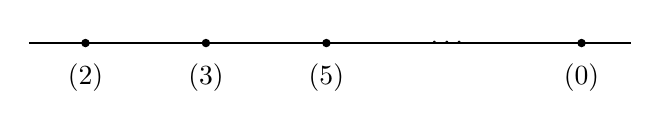
\begin{tikzpicture}[scale=0.9]
  \draw[thick] (-0.8,0) -- (7.7,0);
  \fill (0,0) circle (1.7pt) node[below=4pt] {$(2)$};
  \fill (1.7,0) circle (1.7pt) node[below=4pt] {$(3)$};
  \fill (3.4,0) circle (1.7pt) node[below=4pt] {$(5)$};
  \node at (5.1,0) {$\cdots$};
  \fill (7.0,0) circle (1.7pt) node[below=4pt] {$(0)$};
\end{tikzpicture}
\caption{$\Spec\mathbb{Z}$ 的「一幅图」，看起来与图~\ref{fig:a1c-picture} 可疑地相像。（依原书手绘图重绘。）}\label{fig:spec-z-picture}
\end{figure}

让我们毫无愧色地把关于函数的那套讨论照搬到这个空间上。$100$ 是 $\Spec\mathbb{Z}$ 上的一个函数。它在 $(3)$ 处的值是「$1\pmod{3}$」；它在 $(2)$ 处的值是「$0\pmod{2}$」，而且实际上是一个二重零点。$\frac{27}{4}$ 是 $\Spec\mathbb{Z}$ 上的一个「\trRationalFunction」，在 $(2)$ 之外处处有定义。我们想说：它在 $(2)$ 处有一个二重\trPole，在 $(3)$ 处有一个三重零点。它在 $(5)$ 处的值为
\[
27\times 4^{-1}\equiv 2\times(-1)\equiv 3\pmod{5}.
\]
（我们会随着时间的推移逐步把这段讨论精确化。）

\textbf{例~4（幼稚但重要的例子，外加德语里的「培根」一词）：}\footnote{译注：这个标题在玩谐音梗——德语 \emph{Speck} 意为「培根」，读音正似 $\Spec k$（「speck」）。}$k$ 为任一\trField{}时，集合 $\Spec k$ 无聊得很：一个点。$\Spec 0$（其中 $0$ 是\trZeroRing）则是空集，因为 $0$ 没有\trPrimeIdeal。

\begin{exercise}[关于小概形的小练习]\label{ex:small-schemes-dual-numbers}
(a)~描述集合 $\Spec k[\epsilon]/(\epsilon^2)$。环 $k[\epsilon]/(\epsilon^2)$ 称为\textbf{\trDualNumbers{}环}（ring of dual numbers），日后会显得相当有用。你应当把 $\epsilon$ 想成一个非常小的数，小到它的平方是 $0$（虽然它本身不是 $0$）。它是一个非零函数，却在所有点上都取值为零——这给了我们的第一个「函数并不由其在各点处的值决定」的例子。我们将在 \S3.2.12 中进一步讨论这个现象。

(b)~描述集合 $\Spec k[x]_{(x)}$（关于\trLocalization{}的讨论见 \S1.2.3）。从 \S3.2.9 与练习~3.4.K 开始，我们会反复遇见这个概形。日后你或许会把它看作一条相当好的「光滑曲线」的一片碎片。
\end{exercise}

在例~2 中我们把情形限制在\trAlgClosedField，这是有原因的：若域不是代数闭的，事情会更加微妙。

\textbf{例~5（$\mathbb{R}$ 上的\trAffineLine）：}$\mathbb{A}^1_{\mathbb{R}}=\Spec\mathbb{R}[x]$。利用 $\mathbb{R}[x]$ 是\textbf{\trEuclideanDomain}（Euclidean domain）这一事实，与例~1--3 类似的论证表明：其\trPrimeIdeal{}为 $(0)$、$(x-a)$（$a\in\mathbb{R}$），以及 $(x^2+ax+b)$（其中 $x^2+ax+b$ 是\trIrreducible{}的二次式）。后两类都是\trMaximalIdeal，也就是说，对它们取商皆得\trField。例如：$\mathbb{R}[x]/(x-3)\cong\mathbb{R}$，$\mathbb{R}[x]/(x^2+1)\cong\mathbb{C}$。

\begin{exercise}[不重要练习]\label{ex:irreducible-quadratic-quotient-c}
证明：对最后一类形如 $(x^2+ax+b)$ 的素理想，其商总同构于 $\mathbb{C}$。
\end{exercise}

这样我们就有了实直线上本来就会指望见到的那些点，它们对应实数；有\trGenericPoint{} $0$；还有新的点，我们可以把它们解释为复数的\emph{\trConjugate{}对}（conjugate pairs）（即那个二次式的根）。这最后一类点应当被看作与实数、而非与\trGenericPoint{}更亲近。你可以把 $\mathbb{A}^1_{\mathbb{R}}$ 想象成沿实轴对折起来的复平面。但关键在于：\trGalois{}\trConjugate{}的点（比如 $i$ 与 $-i$）被视为粘在一起。

我们来探索这个空间上的函数。考虑函数 $f(x)=x^3-1$。它在点 $[(x-2)]$ 处的值是 $7$，或者说得更妥帖些，「$7\pmod{x-2}$」。那么在 $(x^2+1)$ 处呢？我们得到
\[
x^3-1\equiv -x-1\pmod{x^2+1},
\]
而这可以卓有成效地解释为 $-i-1$。

本例的一个寓意是：只要愿意，我们可以在非代数闭的域上工作。这固然更复杂，但我们所关心的信息大半仍能找回。

\begin{exercise}[重要练习]\label{ex:affine-line-over-q}
描述集合 $\mathbb{A}^1_{\mathbb{Q}}$。（要画出类似 $\mathbb{A}^1_{\mathbb{R}}$ 那样的图更难。但如图~\ref{fig:a1c-picture} 那样「在一条直线上撒点」的粗略漫画，仍不失为一幅合理的草图。）
\end{exercise}

\textbf{例~6（$\mathbb{F}_p$ 上的\trAffineLine）：}$\mathbb{A}^1_{\mathbb{F}_p}=\Spec\mathbb{F}_p[x]$。与前几例一样，$\mathbb{F}_p[x]$ 是\trEuclideanDomain，故其\trPrimeIdeal{}形如 $(0)$ 或 $(f(x))$，其中 $f(x)\in\mathbb{F}_p[x]$ 是一个次数任意的\trIrreducible{}多项式。\trIrreducible{}多项式对应于 $\mathbb{F}_p$ 上的若干\trGalois{}\trConjugate{}点集。

注意，$\Spec\mathbb{F}_p[x]$ 有 $p$ 个点对应于 $\mathbb{F}_p$ 的元素，但还有多得多的点（无穷多，见\cref{ex:spec-kx-infinite}）。这使得这个空间远比「$p$ 个点」丰富。例如，多项式 $f(x)$ 并不由其在 $\mathbb{F}_p$ 的 $p$ 个元素上的值决定，但它\emph{确实}由其在 $\Spec\mathbb{F}_p[x]$ 的各点处的值决定。（如我们先前所说，这并非对所有概形成立。）

即便你是搞几何的人，也应当琢磨琢磨这件事——这种直觉日后会在几何情形中再现。哪怕你自以为只对在\trAlgClosedField{}（比如 $\mathbb{C}$）上工作感兴趣，也终会被迫面对非代数闭的域（比如 $\mathbb{C}(x)$）。

\begin{exercise}\label{ex:spec-kx-infinite}
若 $k$ 是\trField，证明 $\Spec k[x]$ 有无穷多个点。（提示：\trn{Euclid}{欧几里得}关于 $\mathbb{Z}$ 的素数无穷的证明。）
\end{exercise}

\textbf{例~7（复仿射平面）：}$\mathbb{A}^2_{\mathbb{C}}=\Spec\mathbb{C}[x,y]$。（与例~1、例~2 一样，把 $\mathbb{C}$ 换成\emph{任何}\trAlgClosedField，我们的讨论照样适用。）可惜，$\mathbb{C}[x,y]$ 不是\trPID：$(x,y)$ 不是一个主理想。我们可以很快叫出\emph{一些}\trPrimeIdeal{}的名字。其一是 $(0)$，它同前几例中的诸 $(0)$ 味道相仿。$(x-2,\,y-3)$ 是素的，而且甚至是极大的，因为 $\mathbb{C}[x,y]/(x-2,\,y-3)\cong\mathbb{C}$，这个同构由 $f(x,y)\mapsto f(2,3)$ 给出。更一般地，对任意 $(a,b)\in\mathbb{C}^2$，$(x-a,\,y-b)$ 都是素的。此外，若 $f(x,y)$ 是\trIrreducible{}多项式（例如 $y-x^2$ 或 $y^2-x^3$），则 $(f(x,y))$ 是素的。

\begin{exercise}\label{ex:prime-ideals-cxy}
证明我们已经找全了 $\mathbb{C}[x,y]$ 的\trPrimeIdeal。提示：设 $\mathfrak{p}$ 是一个非主的\trPrimeIdeal。证明可以找到无公因子的 $f(x,y)$ 与 $g(x,y)$，二者都含于 $\mathfrak{p}$。考虑\trEuclideanDomain{} $\mathbb{C}(x)[y]$ 中的欧几里得算法，证明可以找到非零的 $h(x)\in(f(x,y),\,g(x,y))\subset\mathfrak{p}$。利用素性，证明 $h(x)$ 的某个线性因子（比如说 $(x-a)$）位于 $\mathfrak{p}$ 中。同理证明存在某个 $(y-b)\in\mathfrak{p}$。
\end{exercise}

\begin{figure}[htbp]
\centering
\begin{tikzpicture}[scale=1.0]
  \draw[gray!60,thick,->] (-2.8,0) -- (3.0,0);
  \draw[gray!60,thick,->] (0,-2.3) -- (0,2.5);
  \draw[thick] (-1.9,2.3) .. controls (-1.0,1.2) and (-0.5,0.5) .. (0.3,0.55)
    .. controls (1.0,0.6) and (1.05,1.5) .. (0.45,1.62)
    .. controls (-0.05,1.72) and (-0.4,1.15) .. (0.15,0.85)
    .. controls (0.8,0.55) and (1.6,-0.4) .. (2.45,-1.3);
  \fill (-1.7,-0.6) circle (1.9pt);
  \node[anchor=north east,align=right] at (-1.55,-0.72)
    {$(a,b)=[(x-a,\,y-b)]$\\「闭点」（见定义~3.6.8）};
  \node at (1.15,1.35) {$\cdots$};
  \fill (1.6,1.5) circle (1.9pt);
  \node[anchor=west] at (1.72,1.1) {$[(f(x,y))]$};
  \node[anchor=east] at (1.55,-1.55) {$[(0)]$};
  \fill (1.82,-1.45) circle (0.55pt);
  \fill (1.98,-1.25) circle (0.95pt);
  \fill (2.2,-0.95) circle (1.5pt);
\end{tikzpicture}
\caption{画出 $\mathbb{A}^2_{\mathbb{C}}=\Spec\mathbb{C}[x,y]$。（依原书手绘图重绘。）}\label{fig:a2c-picture}
\end{figure}

现在我们试着画出 $\mathbb{A}^2_{\mathbb{C}}$ 的图（见图~\ref{fig:a2c-picture}）。$\mathbb{C}[x,y]$ 的极大素理想对应于 $\mathbb{C}^2$ 中的传统点：$[(x-a,\,y-b)]$ 对应于 $(a,b)\in\mathbb{C}^2$。现在我们得把「附赠点」也想象出来。$[(0)]$ 不知怎地栖身于所有传统点的背后；它在仿射平面的某处，却又不在任何特定的地方。例如，它并不落在抛物线 $y=x^2$ 上。点 $[(y-x^2)]$ 落在抛物线 $y=x^2$ 上，却又不在抛物线的任何特定位置上。（图~\ref{fig:a2c-picture} 有点误导。比如，点 $[(0)]$ 并不在第四象限；它不知怎地邻近其他每一个点，这就是为什么图中把它画成一个略微发散的大点。）从这幅图你能看出，我们其实已经在暗地里思考「维数」了。\trPrimeIdeal{} $(x-a,\,y-b)$ 不知怎地是 $0$ 维的，\trPrimeIdeal{} $(f(x,y))$ 是 $1$ 维的，而 $(0)$ 是 $2$ 维的。（我们在这里谈的维数全是\emph{复}维数或\emph{代数}维数。复平面 $\mathbb{C}^2$ 的实维数是 $4$，复维数是 $2$。复维数一般是实维数的一半。）要到第 12 章我们才会精确定义\trDimension，但在那之前你尽管把它记在心上。

还要注意：\trMaximalIdeal{}对应于「最小」的点。更小的理想对应「更大」的点。「一个\trPrimeIdeal{}包含另一个」说的是那些点「具有相反的包含关系」。等我们有了\trTopology，这一切都会变得精确。这种序的反转有点令人困惑，而且即便在概念精确化之后也仍会如此。

现在我们来看例~7 的显然推广。

\textbf{例~8（复仿射 $n$ 空间——重要！）：}令 $\mathbb{A}^n_{\mathbb{C}}:=\Spec\mathbb{C}[x_1,\dots,x_n]$。（重要定义：更一般地，$\mathbb{A}^n_A$ 定义为 $\Spec A[x_1,\dots,x_n]$，其中 $A$ 是任意\trRing。当基环在上下文中清楚时，下标 $A$ 常被省去。给学究的一句：记号 $\mathbb{A}^n_A$ 隐含地包括了 $n$ 个\textbf{\trCoordinate{}函数}（coordinate functions）$x_1,\dots,x_n$ 这份数据。）为具体起见，取 $n=3$。于是一个起初看似纯代数的问题变得有趣起来：$\mathbb{C}[x,y,z]$ 的\trPrimeIdeal{}是什么？

与之前类似，$(x-a,\,y-b,\,z-c)$ 是一个\trPrimeIdeal。它是\trMaximalIdeal，因为其\trResidueRing{}（residue ring）是一个\trField{}（即 $\mathbb{C}$）；我们把这些点看作「零维点」。基于对这些理想的几何解释，我们将经常把 $[(x-a,\,y-b,\,z-c)]$ 写作 $(a,b,c)$。不会再有别的\trMaximalIdeal{}了，依据是\trHilbert{}弱\trNullstellensatz（\cref{thm:hilbert-weak-nullstellensatz}）。

\vkthmsync{5}
\begin{theorem}[\trHilbert{}弱\trNullstellensatz]\label{thm:hilbert-weak-nullstellensatz}
若 $k$ 是\trAlgClosedField，则 $k[x_1,\dots,x_n]$ 的\trMaximalIdeal{}恰是形如 $(x_1-a_1,\dots,x_n-a_n)$（其中 $a_i\in k$）的那些\trIdeal。
\end{theorem}

我们不妨顺手把一个略强的版本也在此陈述了。

\begin{theorem}[\trHilbert{}\trNullstellensatz]\label{thm:hilbert-nullstellensatz}
若 $k$ 是任意\trField，则 $k[x_1,\dots,x_n]$ 的每个\trMaximalIdeal{}的\trResidueField{}都是 $k$ 的\trFiniteFieldExtension。翻译一下：任何域扩张，只要作为 $k$-代数是有限生成的，就必然作为 $k$-向量空间也是有限生成的（即它是域的\trFiniteFieldExtension）。
\end{theorem}

这条陈述也常被称作\trZariski{}引理。

\begin{exercise}\label{ex:hilbert-nullstellensatz-implies-weak}
证明\trNullstellensatz（\cref{thm:hilbert-nullstellensatz}）蕴含弱\trNullstellensatz（\cref{thm:hilbert-weak-nullstellensatz}）。
\end{exercise}

我们将在 \S8.4.3 证明\trNullstellensatz，并在练习~12.2.B 中再证一次。

下面这个事实是\trNullstellensatz{}的有用搭档。

\begin{exercise}[无须\trNullstellensatz]\label{ex:finite-algebra-domain-field}
任何是有限 $k$-代数的\trIntegralDomain{} $A$（即作为 $k$-向量空间有限维的 $k$-代数）必是\trField。提示：对任意非零 $x\in A$，证明 $\times x\colon A\to A$ 是\trIsomorphism。（于是，与\cref{thm:hilbert-nullstellensatz}相结合便知：\emph{具有有限维剩余环的 $k[x_1,\dots,x_n]$ 的\trPrimeIdeal，恰同于 $k[x_1,\dots,x_n]$ 的\trMaximalIdeal。}这一点值得记住。）
\end{exercise}

$\mathbb{C}[x,y,z]$ 还有别的\trPrimeIdeal。我们有 $(0)$，它对应一个「三维点」。我们有 $(f(x,y,z))$，其中 $f$ \trIrreducible；与之相联系的是「\trHypersurface」（hypersurface）$f=0$，所以这一类在本性上是「二维」的。但我们并没有找全它们！一条线索：我们有了「维数」$0$、$2$、$3$ 的\trPrimeIdeal——还缺「维数 $1$」。这样的一个\trPrimeIdeal{}便是 $(x,y)$。我们把它描绘成 $x=y=0$ 的\trLocus，即 $z$-轴。它是一个\trPrimeIdeal，因为相应的商 $\mathbb{C}[x,y,z]/(x,y)\cong\mathbb{C}[z]$ 是\trIntegralDomain（而且应当被解释为 $z$-轴上的函数）。「一维素理想」有很多，而且没有办法以合理的方式将它们分类。日后会看到，它们对应于我们视为\trIrreducible{}曲线的东西。于是，这个纯代数问题（「$\mathbb{C}[x,y,z]$ 的\trPrimeIdeal{}是什么」）的答案竟然在根本上是几何的！

$\mathbb{A}^1_{\mathbb{Q}}$ 中对应于环 $\mathbb{Q}[x]$ 的\trMaximalIdeal{}的那些点（我们很快会称之为「\trClosedPoint」；见定义~3.6.8）可以解释为 $\overline{\mathbb{Q}}$ 中把\trGalois{}共轭点粘合起来的点（\cref{ex:affine-line-over-q}）；这一事实可推广到 $\mathbb{A}^n_{\mathbb{Q}}$。例如在 $\mathbb{A}^2_{\mathbb{Q}}$ 中，$(\sqrt{2},\sqrt{2})$ 与 $(-\sqrt{2},-\sqrt{2})$ 粘在一起，但与 $(\sqrt{2},-\sqrt{2})$ 不粘。下面的练习会让你略微体会这是怎么回事。

\begin{exercise}\label{ex:maximal-ideals-sqrt2}
描述 $\mathbb{Q}[x,y]$ 中对应于 $(\sqrt{2},\sqrt{2})$ 与 $(-\sqrt{2},-\sqrt{2})$ 的\trMaximalIdeal。再描述 $\mathbb{Q}[x,y]$ 中对应于 $(\sqrt{2},-\sqrt{2})$ 与 $(-\sqrt{2},\sqrt{2})$ 的\trMaximalIdeal。两种情形下的\trResidueField{}各是什么？
\end{exercise}

$\mathbb{A}^2_{\mathbb{Q}}$ 的「\trClosedPoint」（即对应于环 $\mathbb{Q}[x,y]$ 的\trMaximalIdeal{}的那些点）可以描述为 $\overline{\mathbb{Q}}^2$ 中各点的\trGalois{}轨道；这套描述甚至可以推广到其他「非闭」点上，如下。

\begin{exercise}[不重要但棘手而有趣的练习]\label{ex:map-c2-a2q}
考虑集合的映射 $\phi\colon\mathbb{C}^2\to\mathbb{A}^2_{\mathbb{Q}}$，定义如下：$(z_1,z_2)$ 被送到 $\mathbb{Q}[x,y]$ 中由在 $(z_1,z_2)$ 处消失的多项式所组成的\trPrimeIdeal。

(a)~$(\pi,\pi^2)$ 的像是什么？

(b)~\hard\ 证明 $\phi$ 是满射。（警示：你需要一些我们还没讨论过的想法才能解决它。等我们在 $\mathbb{A}^2_{\mathbb{Q}}$ 上定义了\trZariskiTopology，你将能验证 $\phi$ 是\trContinuousMap，其中 $\mathbb{C}^2$ 带的是\trClassicalTopology。这个例子可以推广。比如，日后你也许能把它推广到任意维数。）
\end{exercise}

\textbf{3.2.7.\ 商与局部化。}\quad 从旧环得到新环的两条自然途径——取商与取局部化——在谱的语言中有其解读。

\textbf{3.2.8.\ 商：$\Spec A/I$ 作为 $\Spec A$ 的子集。}\quad 一个重要的事实是：$A/I$ 的\trPrimeIdeal{}与 $A$ 的包含 $I$ 的\trPrimeIdeal{}成双射。

\begin{exercise}[必做代数练习：此前从未见过则必做]\label{ex:quotient-primes-bijection}
设 $A$ 是\trRing，$I$ 是 $A$ 的一个\trIdeal。令 $\phi\colon A\to A/I$。证明 $\phi^{-1}$ 给出 $A/I$ 的\trPrimeIdeal{}与 $A$ 的包含 $I$ 的\trPrimeIdeal{}之间保持包含关系的双射。于是我们可以把 $\Spec A/I$ 描画为 $\Spec A$ 的一个子集。
\end{exercise}

作为一个重要的动机性特例，你如今便有了\emph{仿射复簇}（affine complex varieties）的一幅图景。设 $A$ 是有限生成的 $\mathbb{C}$-代数，由 $x_1,\dots,x_n$ 生成，带关系 $f_1(x_1,\dots,x_n)=\cdots=f_r(x_1,\dots,x_n)=0$。那么这套「生成元与关系」的描述自然让我们能把 $\Spec A$ 解释为 $\mathbb{A}^n_{\mathbb{C}}$ 的一个子集——我们把它想成「传统点」（复数的 $n$ 元组）连同一些我们尚未完全描述的「附赠点」。要看哪些传统点落在 $\Spec A$ 里，只需解方程 $f_1=\cdots=f_r=0$。例如，$\Spec\mathbb{C}[x,y,z]/(x^2+y^2-z^2)$ 可以画作图~\ref{fig:cone-picture} 的模样。（诚然这只是「$\mathbb{R}$-点的草图」，但日后我们仍会觉得它有用。）整幅图景（连同\trNullstellensatz{}一起）在把 $\mathbb{C}$ 换成任何\trAlgClosedField{}后照搬无误。的确，对大多数\trAlgClosedField{} $k$，图~\ref{fig:cone-picture} 也可以说画的是 $\Spec k[x,y,z]/(x^2+y^2-z^2)$（尽管在特征 $2$ 时它有误导性，因为碰巧有 $x^2+y^2-z^2=(x+y+z)^2$）。

\begin{figure}[htbp]
\centering
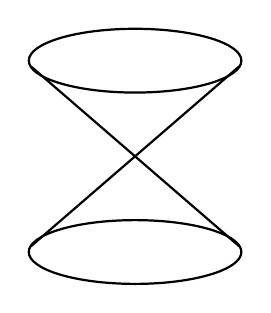
\begin{tikzpicture}[scale=0.9]
  \draw[thick] (0,1.35) ellipse (1.5 and 0.45);
  \draw[thick] (0,-1.35) ellipse (1.5 and 0.45);
  \draw[thick] (-1.47,1.27) -- (1.47,-1.27);
  \draw[thick] (1.47,1.27) -- (-1.47,-1.27);
\end{tikzpicture}
\caption{$\Spec\mathbb{C}[x,y,z]/(x^2+y^2-z^2)$ 的「一幅图」。（依原书手绘图重绘。）}\label{fig:cone-picture}
\end{figure}

\textbf{3.2.9.\ 局部化：$\Spec S^{-1}A$ 作为 $\Spec A$ 的子集。}\quad 下面的练习展示\trPrimeIdeal{}在局部化下的行为。

\begin{exercise}[必做代数练习：此前从未见过则必做]\label{ex:localization-primes-bijection}
设 $S$ 是 $A$ 的\trMultiplicativeSubset。描述 $S^{-1}A$ 的\trPrimeIdeal{}与 $A$ 中\emph{不与}\trMultiplicativeSubset{} $S$ 相交的\trPrimeIdeal{}之间保持序的双射。
\end{exercise}

回忆 \S1.2.3：局部化有两种重要的风味。第一种是 $A_f=\{1,f,f^2,\dots\}^{-1}A$，其中 $f\in A$；一个动机性的例子是 $A=\mathbb{C}[x,y]$、$f=y-x^2$。第二种是 $A_{\mathfrak{p}}=(A\smallsetminus\mathfrak{p})^{-1}A$，其中 $\mathfrak{p}$ 是\trPrimeIdeal；动机性的例子：$A=\mathbb{C}[x,y]$、$S=A\smallsetminus(x,y)$。

若 $S=\{1,f,f^2,\dots\}$，则 $S^{-1}A$ 的\trPrimeIdeal{}恰是那些不包含 $f$ 的\trPrimeIdeal——也就是「$f$ 不消失」的那些点。（在 \S3.5 中，等我们知道了\trOpenSet{}是什么，就会把这样的东西称作\emph{\trDistinguishedOpen}（distinguished open set）。）于是要画出 $\Spec\mathbb{C}[x,y]_{y-x^2}$，就先画仿射平面，然后扔掉抛物线 $y-x^2=0$ 上的那些点——即诸点 $(a,a^2)$（$a\in\mathbb{C}$）（意思是 $[(x-a,\,y-a^2)]$），以及「新一类的点」$[(y-x^2)]$。

思考「倒转\trZerodivisor」情形下的局部化，起初可能令人困惑，因为此时局部化 $A\to S^{-1}A$ 不是\trInjectiveMap（\cref{ex:when-localization-is-injective}）。几何直观能帮上忙。考虑 $A=\mathbb{C}[x,y]/(xy)$、$f=x$ 的情形。局部化 $A_f$ 是什么？空间 $\Spec\mathbb{C}[x,y]/(xy)$「就是」仿射平面中两条坐标轴之并。局部化意味着扔掉 $x$ 消失的\trLocus。于是剩下的就是 $x$-轴挖去原点，因此我们预期得到 $\Spec\mathbb{C}[x]_x$。所以应当有某个自然的\trIsomorphism
\[
(\mathbb{C}[x,y]/(xy))_x\stackrel{\ \sim\ }{\longrightarrow}\mathbb{C}[x]_x.
\]

\begin{exercise}\label{ex:xy-localization-isomorphism}
证明这两个环同构。（你将看到，左边的 $y$ 到了右边变成 $0$。）
\end{exercise}

若 $S=A\smallsetminus\mathfrak{p}$，则 $S^{-1}A$ 的\trPrimeIdeal{}恰是 $A$ 的含于 $\mathfrak{p}$ 的那些\trPrimeIdeal。在我们的例子 $A=\mathbb{C}[x,y]$、$\mathfrak{p}=(x,y)$ 中，我们保留所有对应于「穿过原点的东西」的点，即零维点 $(x,y)$、二维点 $(0)$，以及满足 $f(0,0)=0$ 的一维点 $(f(x,y))$，也就是那些「穿过原点的\trIrreducible{}曲线」。你可以把这想象成原点近旁平面的一片碎片；凡在原点处实际上「看不见」的东西都被丢弃（见图~\ref{fig:shred-of-a2}）。

\begin{figure}[htbp]
\centering
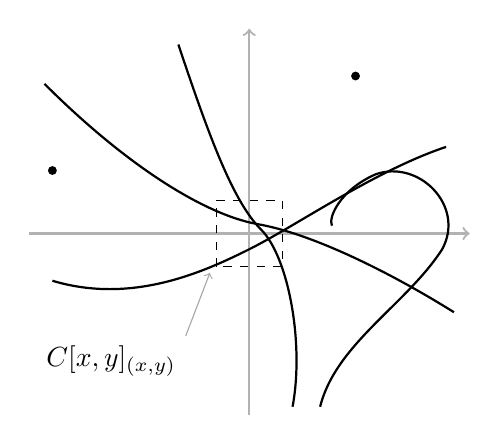
\begin{tikzpicture}[scale=1.0]
  \draw[gray!60,thick,->] (-2.8,0) -- (2.8,0);
  \draw[gray!60,thick,->] (0,-2.3) -- (0,2.6);
  \draw[thick] (-0.9,2.4) .. controls (-0.5,1.2) and (-0.2,0.4) .. (0.15,0.05)
    .. controls (0.5,-0.3) and (0.7,-1.4) .. (0.55,-2.2);
  \draw[thick] (-2.6,1.9) .. controls (-1.6,0.9) and (-0.6,0.25) .. (0.1,0.12)
    .. controls (0.8,0.0) and (1.8,-0.5) .. (2.6,-1.0);
  \draw[thick] (-2.5,-0.6) .. controls (-1.5,-0.9) and (-0.6,-0.5) .. (0.0,-0.2)
    .. controls (0.6,0.1) and (1.6,0.8) .. (2.5,1.1);
  \draw[thick] (0.9,-2.2) .. controls (1.1,-1.4) and (2.0,-0.9) .. (2.45,-0.2)
    .. controls (2.75,0.35) and (2.15,0.95) .. (1.6,0.75)
    .. controls (1.15,0.55) and (1.0,0.2) .. (1.05,0.1);
  \draw[dashed] (-0.42,-0.42) rectangle (0.42,0.42);
  \fill (1.35,2.0) circle (1.6pt);
  \fill (-2.5,0.8) circle (1.6pt);
  \node[anchor=north west] (speclab) at (-2.7,-1.3) {$\Spec \mathbb{C}[x,y]_{(x,y)}$};
  \draw[gray!70,->] (speclab.north east) -- (-0.5,-0.5);
\end{tikzpicture}
\caption{把 $\Spec \mathbb{C}[x,y]_{(x,y)}$ 画作「$\mathbb{A}^2_{\mathbb{C}}$ 的一片碎片」：只剩下原点附近的那些点。（依原书手绘图重绘。）}\label{fig:shred-of-a2}
\end{figure}

另一个例子：$A=k[x]$、$\mathfrak{p}=(x)$（或者更一般地，$\mathfrak{p}$ 是任一\trMaximalIdeal）。此时 $A_{\mathfrak{p}}$ 只有两个\trPrimeIdeal（\cref{ex:small-schemes-dual-numbers}(b)）。你应当把它看作一条「光滑曲线」的\trGerm：其中一个点是「经典点」，另一个点则是「曲线的\trGenericPoint」。这是\trDVR{}（discrete valuation ring）的一个例子；而事实上，一切\trDVR{}都应当这样来直观化。我们将在 \S13.5 讨论\trDVR。到那时，「光滑」与「曲线」这两个词的用法都将得到辩护。（现实检验：试着把 $\mathbb{Z}$ 在 $(2)$ 处与在 $(0)$ 处的局部化的谱画出来。这两幅图有何不同？）

\textbf{3.2.10.\ 重要事实：环的映射诱导谱的映射（作为集合）。}\quad 我们现在做一条观察，它日后将成长为概形态射的概念。

\begin{exercise}[重要而容易的练习]\label{ex:preimage-of-prime-ideal}
若 $\phi\colon B\to A$ 是环映射，而 $\mathfrak{p}$ 是 $A$ 的一个\trPrimeIdeal，证明 $\phi^{-1}(\mathfrak{p})$ 是 $B$ 的\trPrimeIdeal。
\end{exercise}

于是，环映射 $\phi\colon B\to A$ 诱导一个「方向相反」的集合映射 $\Spec A\to\Spec B$。这给出一个从\trRing{}的\trCategory{}到\trSet{}的\trCategory{}的\trContravariantFunctor：两个环映射的复合诱导相应的谱映射的复合。

\begin{exercise}[容易的练习：现实检验]\label{ex:inclusion-quotient-localization}
设 $B$ 是\trRing。
(a)~设 $I\subset B$ 是一个\trIdeal。证明映射 $\Spec B/I\to\Spec B$ 就是 \S3.2.8 的那个包含。
(b)~设 $S\subset B$ 是乘性子集。证明映射 $\Spec S^{-1}B\to\Spec B$ 就是 \S3.2.9 的那个包含。
\end{exercise}

\textbf{3.2.11.\ 一个显式的例子。}\quad 在「仿射复簇」（或者确实，任何\trAlgClosedField{}上的仿射簇）的情形，由显式公式给出的映射与环映射之间的翻译相当直接。例如，考虑从 $\mathbb{C}^2$ 中由 $b=a^2$ 给出的抛物线（\trCoordinate{}为 $a$ 与 $b$）到 $\mathbb{C}^3$ 中由方程 $y=x^2$ 与 $z=y^2$ 割出的「曲线」（\trCoordinate{}为 $x$、$y$、$z$）的一个映射。设该映射把点 $(a,b)\in\mathbb{C}^2$ 送到点 $(a,b,b^2)\in\mathbb{C}^3$。在我们的新语言中，我们有一个映射
\[
\Spec \mathbb{C}[a,b]/(b-a^2)\longrightarrow \Spec \mathbb{C}[x,y,z]/(y-x^2,\ z-y^2)
\]
由下式给出：
\[
\mathbb{C}[a,b]/(b-a^2)\longleftarrow\mathbb{C}[x,y,z]/(y-x^2,\ z-y^2),
\]
\[
(a,b,b^2)\longmapsto(x,y,z),
\]
即 $x\mapsto a$、$y\mapsto b$、$z\mapsto b^2$。如果这个想法还不清楚，下面两道练习非常值得做——头一次见到时它们可能极其令人困惑，而等你终于想通之时，它们又极具启发性（而且是平凡的）。

\begin{figure}[htbp]
\centering
\begin{tikzpicture}[scale=0.9]
  \draw[very thick] (-2.6,-1.7) -- (-2.6,2.4);
  \node at (-2.6,-2.2) {$y$-线};
  \draw[thick] plot[domain=-1.75:1.75,samples=41] ({\x+1.5},{\x*\x-1.6});
  \node at (1.5,-2.2) {$x$-线};
  \draw[gray!70,->] (0.3,0.75) -- (-1.9,0.75);
\end{tikzpicture}
\caption{由 $x\mapsto y=x^2$ 给出的映射 $\mathbb{C}\to\mathbb{C}$。（依原书手绘图重绘。）}\label{fig:parabola-map}
\end{figure}

\begin{exercise}[重要练习：特例]\label{ex:parabola-projection-special-case}
考虑复流形之间的映射 $\mathbb{C}\to\mathbb{C}$，由 $x\mapsto y=x^2$ 给出。我们把「源」$\mathbb{C}$ 解释为「$x$-线」，把「目标」$\mathbb{C}$ 解释为「$y$-线」。你可以把它想象为 $xy$-平面中的抛物线 $y=x^2$ 到 $y$-轴的投影（见图~\ref{fig:parabola-map}）。把相应的环映射解释为由 $y\mapsto x^2$ 给出的 $\mathbb{C}[y]\to\mathbb{C}[x]$。利用上文给出的定义（把 $a$ 与 $[(y-a)]$ 等同，把 $\sqrt{a}$ 与 $[(x-\sqrt{a})]$ 等同），验证点 $a\in\mathbb{C}$ 上方的原像（即\trFiber）是点（们）$\pm\sqrt{a}\in\mathbb{C}$。（本例的一个更成熟的版本出现在例~10.3.4 中。警示：在那里的 $x$ 与 $y$ 角色互换，为的是以某种方式描绘二重覆盖。）
\end{exercise}

\begin{exercise}[重要练习：推广例~3.2.11]\label{ex:polynomial-map-of-spectra}
设 $k$ 是\trField，并给定 $f_1,\dots,f_n\in k[x_1,\dots,x_m]$。令 $\phi\colon k[y_1,\dots,y_n]\to k[x_1,\dots,x_m]$ 是由 $y_i\mapsto f_i$ 定义的 $k$-代数之间的\trMorphism。
(a)~证明：对任意满足 $\phi(J)\subset I$ 的\trIdeal{} $I\subset k[x_1,\dots,x_m]$ 与 $J\subset k[y_1,\dots,y_n]$，$\phi$ 诱导集合的映射 $\Spec k[x_1,\dots,x_m]/I\to\Spec k[y_1,\dots,y_n]/J$。（你不妨先考虑 $I=0$、$J=0$ 的情形。事实上，(a) 与 $k$-代数毫无关系；你也可以在把环 $k[x_1,\dots,x_m]$ 与 $k[y_1,\dots,y_n]$ 换成一般的\trRing{} $A$ 与 $B$ 时证明这条陈述。）
(b)~证明 (a) 中的映射把点 $(a_1,\dots,a_m)\in k^m$（更精确地，$[(x_1-a_1,\dots,x_m-a_m)]\in\Spec k[x_1,\dots,x_m]$）送到
\[
(f_1(a_1,\dots,a_m),\ \dots,\ f_n(a_1,\dots,a_m))\in k^n.
\]
\end{exercise}

\begin{exercise}[练习：画出 $\mathbb{A}^n_{\mathbb{Z}}$]\label{ex:affine-space-over-z-picture}
考虑集合的映射 $\pi\colon\mathbb{A}^n_{\mathbb{Z}}\to\Spec\mathbb{Z}$，由环映射 $\mathbb{Z}\to\mathbb{Z}[x_1,\dots,x_n]$ 给出。若 $p$ 是素数，请描述纤维 $\pi^{-1}([(p)])$ 与 $\mathbb{A}^n_{\mathbb{F}_p}$ 之间的双射。（你无须描述这两个集合中的任何一个！这倒是好事，因为你根本办不到。）本练习也许会让你体味到该如何描绘映射（见图~\ref{fig:an-over-z-family}），尤其是为什么你可以把 $\mathbb{A}^n_{\mathbb{Z}}$ 想成 $\Spec\mathbb{Z}$ 上的一个「$\mathbb{A}^n$-丛」。（你能把 $[(0)]$ 之上的纤维解释成某个域 $k$ 的 $\mathbb{A}^n_k$ 吗？）
\end{exercise}

\begin{figure}[htbp]
\centering
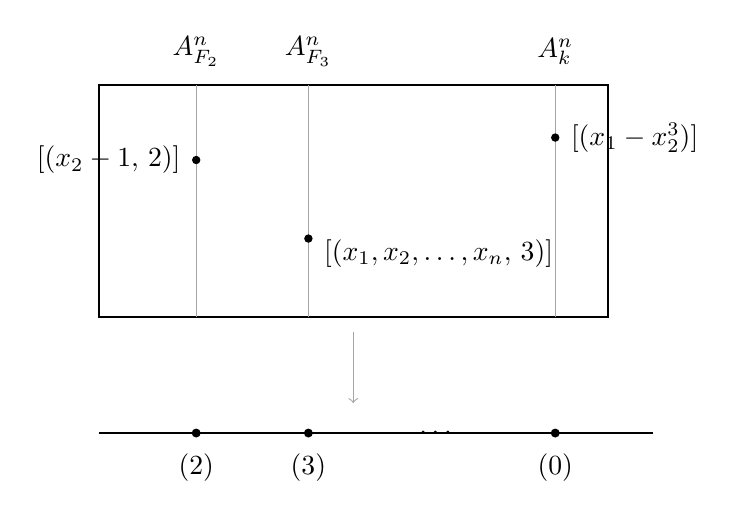
\begin{tikzpicture}[scale=0.95]
  \node at (0.4,2.65) {$\mathbb{A}^n_{\mathbb{F}_2}$};
  \node at (1.9,2.65) {$\mathbb{A}^n_{\mathbb{F}_3}$};
  \node at (5.2,2.65) {$\mathbb{A}^n_{k}$};
  \draw[thick] (-0.9,-0.9) rectangle (5.9,2.2);
  \draw[gray!70] (0.4,2.2) -- (0.4,-0.9);
  \draw[gray!70] (1.9,2.2) -- (1.9,-0.9);
  \draw[gray!70] (5.2,2.2) -- (5.2,-0.9);
  \fill (0.4,1.2) circle (1.6pt);
  \node[anchor=east] at (0.32,1.2) {$[(x_2-1,\,2)]$};
  \fill (1.9,0.15) circle (1.6pt);
  \node[anchor=west] at (1.98,-0.05) {$[(x_1,x_2,\dots,x_n,\,3)]$};
  \fill (5.2,1.5) circle (1.6pt);
  \node[anchor=west] at (5.28,1.5) {$[(x_1-x_2^3)]$};
  \draw[gray!70,->] (2.5,-1.1) -- (2.5,-2.05);
  \draw[thick] (-0.9,-2.45) -- (6.5,-2.45);
  \fill (0.4,-2.45) circle (1.7pt) node[below=4pt] {$(2)$};
  \fill (1.9,-2.45) circle (1.7pt) node[below=4pt] {$(3)$};
  \node at (3.6,-2.45) {$\cdots$};
  \fill (5.2,-2.45) circle (1.7pt) node[below=4pt] {$(0)$};
\end{tikzpicture}
\caption{$\mathbb{A}^n_{\mathbb{Z}}\to\Spec\mathbb{Z}$ 的一幅图：画成「$\mathbb{A}^n$ 之族」，或者说「$\Spec\mathbb{Z}$ 上的 $\mathbb{A}^n$-丛」。$k$ 是什么域？应当怎样「几何地」思考图中标出的三个点？（依原书手绘图重绘。）}\label{fig:an-over-z-family}
\end{figure}

\textbf{3.2.12.\ 函数并不由其在各点处的值决定：这是幂零元之过。}\quad 本节我们以描述一些古怪的行为作结。我们正在发展一套机器，它将让我们得以把几何直观带进代数。有一处十分十分要紧的地方，你的直觉在那里会是错的，所以你现在就该知道这件事，并相应地调整你的直觉。正如\trMumford{}（[Mu2, p.~12]）所指出的：「概形的这个侧面，在\trGrothendieck{}定义它们之时是最为惊世骇俗的。」

设我们有一个在所有点处都消失的函数（环元素）。那么它未必是零函数！这个问题的翻译是：全体\trPrimeIdeal{}的交是否必然恰好是 $0$？答案是否定的，对\trDualNumbers{}环 $k[\epsilon]/(\epsilon^2)$ 这个例子便是明证：$\epsilon\neq0$，但 $\epsilon^2=0$。（我们在\cref{ex:small-schemes-dual-numbers}(a) 中见过这个环。）任何某次幂为零的函数自然落在全体\trPrimeIdeal{}的交之中。

\begin{exercise}\label{ex:nilpotents-and-nilradical}
某次幂为 $0$ 的环元素称为\textbf{\trNilpotent{}元}（nilpotents）。
(a)~证明：若 $I$ 是由\trNilpotent{}元组成的\trIdeal，则 \cref{ex:quotient-primes-bijection} 中的包含 $\Spec B/I\to\Spec B$ 是双射。于是\trNilpotent{}元不影响底集合。（我们很快将在 \S3.4.7 中看到，它们也不影响\trTopology——差别将在\trStructureSheaf{}之中。）
(b)~证明\trRing{} $B$ 的全体\trNilpotent{}元构成一个\trIdeal。这个\trIdeal{}称为\textbf{\trNilradical}（nilradical），记作 $\mathfrak{N}=\mathfrak{N}(B)$。
\end{exercise}

于是\trNilradical{}含于全体\trPrimeIdeal{}的交之中。逆命题也真：

\vkthmsync{13}
\begin{theorem}\label{thm:nilradical-intersection-primes}
\trNilradical{} $\mathfrak{N}(A)$ 是 $A$ 的全部\trPrimeIdeal{}的交。几何地说：$\Spec A$ 上的一个函数在每一点处都消失，当且仅当它是\trNilpotent{}的。
\end{theorem}

\begin{exercise}\label{ex:nilradical-theorem-proof}
如果你不知道这条定理，那就去查一查，或者更好的是，亲自证它。（提示：利用「$A$ 的任何\trProperIdeal{}都含于某个\trMaximalIdeal」这一事实，而这需要\trZornsLemma。可能的进一步提示：设 $x\notin\mathfrak{N}(A)$。我们要证明存在不含 $x$ 的\trPrimeIdeal。证明 $A_x$ 不是\trZeroRing，办法是证明 $1\neq0$。）
\end{exercise}

\textbf{3.2.14.}\quad 特别地，尽管「函数并不由其在各点处的值决定」令人不安，但我们已经把这种直觉失灵的确切内容指了出来：两个函数在各点处取值相同，当且仅当它们相差一个\trNilpotent{}元。你应当从几何上思考这件事：一个函数在\trRing{}的谱的每一点处都消失，当且仅当它有一次幂为零。而如果没有非零\trNilpotent{}元——若 $\mathfrak{N}=(0)$——那么函数\emph{确实}由其在各点处的值决定。如果一个\trRing{}没有非零\trNilpotent{}元，我们就称它是\textbf{\trReduced}（reduced）的。

\begin{exercise}[有趣的不重要练习：不用 $\delta$ 与 $\epsilon$ 的求导——至少不用 $\delta$]\label{ex:derivatives-dual-numbers}
设有多项式 $f(x)\in k[x]$。我们改在 $k[x,\epsilon]/(\epsilon^2)$ 中工作。那么 $f(x+\epsilon)$ 是什么？（先做几个例子，再证明你观察到的模式。）这是一个暗示：\trNilpotent{}元将在定义微分信息（第 21 章）时十分重要。
\end{exercise}


\section{概形可视化：一般点}

\epigraph
  {从前，人们常郑重其事地警告说：图画不严格；这一吓唬从未被人叫破，
   倒把它的受害者们永远地吓住，使其一味只求稳当。诚然，有些图画并不严格，
   但我得说，大多数图画是严格的（而我自己但凡可行，总要使用它们）。}
  {——J.~E.~\trLittlewood，[Lit, p.~54]}
\epigraph
  {我们都知道，艺术不是真理。艺术是一种谎言，它使我们领悟真理——至少是
   那被赋予我们去理解的真理。艺术家必须懂得以何种方式使人相信他的谎言的
   真实性。}
  {——P.~\trPicasso，[Pi, p.~315]}

多年来，你一直能够在平面中想象 $x^2+y^2=1$，而如今你对如何想象
$\Spec \mathbb{Z}$ 也已有了一些想法。既然我们宣称要（借助 $\Spec$
\trFunctor）把\trRing{}当作几何对象来理解，那么我们就应当希望对这些对象
发展出几何上的洞见。要培养关于\trScheme{}的几何直观，在头脑中备有图画是
有益的——把你对已然熟悉的那些\trGeometricSpace{}所怀的直观延伸过来便是。
随着行文推进，我们会凭经验逐步形成「\trScheme{}应当长成什么模样」的
一些想法。本节便总结我们迄今之所获。

有些数学家宁愿全然代数式地思考，从不以图画的方式想问题。另一些人则会因
这乃是艺术而非科学而心生不安。最后，这类「挥手比划」（hand-waving）式的
议论\footnote{译注：hand-waving，数学行话，指以挥挥手带过细节、不作严格
论证的讲法。}注定绝不会用于理论的严格展开。鉴于这些理由，你或许想跳过
这几节。然而，头脑中若有正确的图画，会大大有助于理解哪些事实应当为真、
又当如何证明它们。\trFitzGerald{}关于拓展心智之重要的那番勉励，是给数学家的
一条要紧忠告。

\epigraph
  {检验一流智力的标准，是看你能否在头脑中同时容纳两种相反的观念，
   而仍不丧失行事的能力。}
  {——F.~Scott~\trFitzGerald，《崩溃》[Fi, p.~41]}

我们的出发点是「仿射复\trVariety」这一例子（即在 $\mathbb{C}$ 上由涉及
有限多个变量的方程切出来的东西），以及更一般地，任意\trAlgClosedField{}
上的类似例子。我们从直观的观念入手（「传统的点」按你所期待的方式行事），
然后再加入两个既新颖又令人不安的特征：\trGenericPoint{}与非\trReduced{}行为。
此后你便可把这个观念拓展到那些貌似不同的空间，例如 $\Spec \mathbb{Z}$。

\trHilbert{}弱\trNullstellensatz（\cref{thm:hilbert-weak-nullstellensatz}）表明，
「传统的点」确实作为\trScheme{}的点而存在，且这一点对任何\trAlgClosedField{}皆然。
若域不是代数闭的，传统的点就会经\trGalois{}\trConjugate{}被粘成一团一团，
正如 \S3.2 中的例~5（实\trAffineLine）与例~6（$\mathbb{F}_p$ 上的%
\trAffineLine）那样。这是\trHilbert{}\trNullstellensatz（\cref{thm:hilbert-nullstellensatz}）
的一个几何解读。

但图中还有一些额外的点有待添入。你应当记住：这些点「对应」于「\trIrreducible」
「闭」的（代数）子集。作为动机，考虑复仿射平面（例~7）的情形：对每个%
\trIrreducible{}多项式，我们都曾有一个这样的点；此外另有一个点对应于整个平面。
当我们（在下一节中）定义\trZariskiTopology{}时，会把「闭」说得精确。
对于「\trIrreducible」应当是什么意思，你或许已有想法；我们将在
\S3.6 的开头把它说精确。所谓「对应」，意思是：每个闭的\trIrreducible{}子集都有
一个相应的点坐在它上面，称为它的\trGenericPoint（定义见 \S3.6）。它是一个新点，与该子集中所有其余的点都不相同。（对
$\Spec A$ 而言，这一对应描述于练习~3.7.F；对一般的\trScheme{}，则描述于
练习~5.1.B。）我们并不知道该把一般点画在何处才算精确，故不妨把它随意搁
在任何地方；但你应当把它想成「几乎处处」都在——特别地，它靠近该子集中
每一个其他的点。

在 \S3.2.8 中，我们曾看到 $\Spec A/I$ 的点应当如何解读为 $\Spec A$ 的
一个子集。所以举例来说，当你见到 $\Spec \mathbb{C}[x,y]/(x+y)$ 时，你不应
只把它想象成一条直线，而应想象成 $xy$ 平面中的一条直线：\trAlgebra{}
$\mathbb{C}[x,y]$ 的生成元 $x$ 与 $y$ 的选取，本身便蕴含了一个到仿射空间
中的\trInclusionMap{}。

在 \S3.2.9 中，我们曾看到 $\Spec S^{-1}A$ 的点应当如何解读为 $\Spec A$ 的
子集。两种最重要的情形都已在彼处讨论过：$\Spec A_f$ 的点对应于 $\Spec A$
中使 $f$ 不消失的点；我们稍后（\S3.5）将把它解读为一个\trDistinguishedOpen。

若 $\mathfrak{p}$ 是一个\trPrimeIdeal{}，则应把 $\Spec A_{\mathfrak{p}}$
看作「空间 $\Spec A$ 在 $\mathfrak{p}$ 所对应子集近旁的一片碎片」。此事
最简单的非平凡情形是 $A=k[x]$ 而 $\mathfrak{p}=(x)\subset A$（见
\cref{ex:small-schemes-dual-numbers}；我们将在练习~3.4.K 中再次讨论它）。

\epigraph
  {「他们中间若有谁能解释它，」爱丽丝说（她在方才这几分钟里已长得
   如此高大，打断他半点也不再害怕），「我就给他六便士。我才不信这里面有
   一丁点儿意思。」

   「这里面若是没有意思，」国王说，「那倒省去了天大的麻烦，你知道的，
   咱们也就不必费心去找了。」}
  {——刘易斯·\trCarroll，[Carr, Ch.~XII]}


\section{仿射概形的底拓扑空间}

接下来，我们将在一个环的\trSpectrum{}上引入\emph{\trZariskiTopology}。这个定义初听之下颇为
古怪，但稍加经验便会觉得合情合理。作为动机，考虑 $\mathbb{A}^2_{\mathbb{C}}=%
\Spec\mathbb{C}[x,y]$，即复（仿射）平面（外加几个额外的点）。在\trAlgebraicGeometry{}中，
我们将只被允许考虑\trAlgebraicFunction，也就是 $x$ 与 $y$ 的多项式。一个多项式
在其中消失的\trLocus，按理应当是一个\trClosedSet；而\trZariskiTopology{}的定义方式，就是规定：
我们应当视为闭的集合，唯有这些集合，以及被它们连带逼成闭的那些集合。换言之，
它是使这些集合成为闭集的最\trCoarse\trTopology。

\textbf{3.4.1.}\quad 特别地，虽然\trTopology{}通常借\trOpenSubset{}来描述，但对我们
而言，以\trClosedSubset{}来定义这个\trTopology{}反而更方便。若 $S$ 是\trRing{} $A$ 的一个子集，
定义 $S$ 的\textbf{\trVanishingSet{}}（vanishing set）为
\[
V(S):=\{\, [\mathfrak{p}]\in\Spec A \;:\; S\subset\mathfrak{p} \,\}.
\]
它是 $S$ 的全部元素在其上都取值为零的那些点所成的集合。（把「在一点处消失」与
「含于一个\trPrimeIdeal{}之中」等同起来，如今应当已成为你的第二天性。）我们宣布：
唯有这些集合——别无其他——才是\trClosedSubset。

例如，考虑 $V(xy,\,yz)\subset\mathbb{A}^3_{\mathbb{C}}=\Spec\mathbb{C}[x,y,z]$。
哪些点含于这个\trLocus？我们把它想成求解 $xy=yz=0$。在「传统点」之中（把它们解读为
复数的三元组，这要多亏\trHilbert{}弱\trNullstellensatz，即%
\cref{thm:hilbert-weak-nullstellensatz}），我们有 $y=0$ 或 $x=z=0$ 的那些点：分别是
$xz$-平面与 $y$-轴。在「新」点之中，我们有 $xz$-平面的\trGenericPoint（亦即点 $[(y)]$），
以及 $y$-轴的\trGenericPoint（亦即点 $[(x,z)]$）。你或许还会想象，我们另有一些含于
$xz$-平面之中的「一维」点。

\begin{exercise}[容易的练习]\label{ex:x-axis-vanishing-locus}
验证 $x$-轴含于 $V(xy,\,yz)$。（$x$-轴由 $y=z=0$ 定义，$y$-轴与 $z$-轴可类似定义。）
\end{exercise}

让我们回到一般情形。下面的练习使我们能把注意力限定在\trIdeal{}的\trVanishingSet{}上。

\begin{exercise}[容易的练习]\label{ex:vanishing-set-generated-ideal}
证明：若 $(S)$ 是由 $S$ 生成的\trIdeal，则 $V(S)=V((S))$。
\end{exercise}

\textbf{3.4.2.}\ \emph{\trhDefinition{}。}\quad 我们如此定义\textbf{\trZariskiTopology}：
宣布对一切 $S$，$V(S)$ 都是闭集。（我们不妨在此顺便声明：\textbf{\trZariskiClosure{}}
（Zariski closure）指\trZariskiTopology{}中的闭包。）我们来验证\trZariskiTopology{}
的确是一个\trTopology：

\begin{exercise}\label{ex:zariski-topology-axioms}
(a)~证明 $\varnothing$ 与 $\Spec A$ 都是 $\Spec A$ 的\trOpenSubset。

(b)~若 $I_i$（$i$ 跑遍某个\trIndexSet）是一族\trIdeal，证明
$\bigcap_i V(I_i)=V\bigl(\sum_i I_i\bigr)$。于是，任意一族\trOpenSet{}的并仍是开的。

(c)~证明 $V(I_1)\cup V(I_2)=V(I_1I_2)$。（$A$ 的两个\trIdeal{} $I_1$ 与 $I_2$ 的%
\textbf{乘积}（product of two ideals），指形如 $\sum_{j=1}^{n}i_{1,j}i_{2,j}$（其中
$i_{k,j}\in I_k$）的有限多条 $A$-线性组合；等价地，它是由 $I_1$ 的元素与 $I_2$ 的
元素的乘积所生成的\trIdeal。你应当迅速核验：这是一个\trIdeal，而且乘积满足结合律，
即 $(I_1I_2)I_3=I_1(I_2I_3)$。）于是，任意有限多个\trOpenSet{}的交仍是开的。
\end{exercise}

\textbf{3.4.3.\ 「\trVanishingSet{}」函数 $V(\cdot)$ 的性质。}\quad 函数 $V(\cdot)$ 显然反转
包含关系：若 $S_1\subset S_2$，则 $V(S_2)\subset V(S_1)$。\trhWarning：可能出现
第二个包含取等号、而第一个不取等号的情形，正如下面的练习所示。

\begin{exercise}[练习兼定义]\label{ex:radical-of-an-ideal}
设 $I\subset A$ 是一个\trIdeal，定义它的\textbf{\trRadical}（radical）为
\[
\sqrt{I}:=\{\, r\in A \;:\; r^n\in I \text{ 对某个 } n\in\mathbb{Z}^{>0} \,\}.
\]
例如，\trNilradical{} $\mathfrak{N}$（\cref{ex:nilpotents-and-nilradical}）就是 $\sqrt{(0)}$。
证明 $\sqrt{I}$ 是一个\trIdeal（参看\cref{ex:nilpotents-and-nilradical}(b)）。证明
$V(\sqrt{I})=V(I)$。若一个\trIdeal{}等于它自身的根，我们就称它是\textbf{\trRadicalIdeal{}}
（radical）。证明 $\sqrt{\sqrt{I}}=\sqrt{I}$，并且\trPrimeIdeal{}都是\trRadicalIdeal{}。
\end{exercise}

下面是两条有用的推论。由于 $(I\cap J)^2\subset IJ\subset I\cap J$（\trIdeal{}的乘积
定义于\cref{ex:zariski-topology-axioms}），我们有 $V(IJ)=V(I\cap J)$（由%
\cref{ex:zariski-topology-axioms}(c)，它又等于 $V(I)\cup V(J)$）。此外，将它与%
\cref{ex:vanishing-set-generated-ideal}相结合，便得
$V(S)=V((S))=V(\sqrt{(S)})$。

\begin{exercise}[练习：根与有限交交换]\label{ex:radicals-finite-intersections}
若 $I_1,\dots,I_n$ 是\trRing{} $A$ 的\trIdeal，证明
$\sqrt{\bigcap_{i=1}^{n}I_i}=\bigcap_{i=1}^{n}\sqrt{I_i}$。日后我们将反复使用这条
性质，而不再回指本练习。
\end{exercise}

\begin{exercise}[留待后用的练习]\label{ex:radical-intersection-primes}
证明 $\sqrt{I}$ 是包含 $I$ 的全部\trPrimeIdeal{}的交。（提示：在一个适当的环上
使用\cref{thm:nilradical-intersection-primes}。）
\end{exercise}

\textbf{3.4.4.\ 例子。}\quad 我们来看看这套机制与前一小节的诸例子如何互相咬合。

回想一下：$\mathbb{A}^1_{\mathbb{C}}$ 作为一个\trSet，本就只有「传统点」（对应于诸%
\trMaximalIdeal，与 $a\in\mathbb{C}$ 成\trBijection），外加一个「新」点 $[(0)]$。
$\mathbb{A}^1_{\mathbb{C}}$ 上的\trZariskiTopology{}不怎么令人激动：诸\trOpenSet{}
就是空集，以及 $\mathbb{A}^1_{\mathbb{C}}$ 挖去有限多个\trMaximalIdeal{}所得的集合。
（它「差点儿」就是\trCofiniteTopology{}（cofinite topology）。注意：诸\trOpenSet{}由它们与
「传统点」的交所决定；「新」点 $[(0)]$ 只是顺路被捎带着走，这是个好兆头，说明它
并无大碍。若无视那个「新」点，便能看到 $\mathbb{A}^1_{\mathbb{C}}$ 上的\trTopology{}比
$\mathbb{C}$ 上的\trClassicalTopology{}更\trCoarse。）

\begin{exercise}\label{ex:topological-space-a1k}
描述\trTopologicalSpace{} $\mathbb{A}^1_k$（参看\cref{ex:spec-kx-infinite}）。
（注意：那个奇怪的
新点 $[(0)]$ 「贴近每一个其他的点」——每个点的每个\trNeighborhood{}都含有 $[(0)]$。
这是这类新点的通性；参看\cref{ex:generic-point-near-every-point}。）
\end{exercise}

$\Spec\mathbb{Z}$ 的情形类似：\trTopology{}以同样的方式「差点儿」是\trCofiniteTopology{}。
诸\trOpenSet{}
是空集，以及 $\Spec\mathbb{Z}$ 挖去有限多个「寻常」素数（即诸点 $(p)$，其中 $p$
为素数）所得的集合。

\textbf{3.4.5.}\ \emph{$\mathbb{A}^2_{\mathbb{C}}$ 的闭子集。}\quad
$\mathbb{A}^2_{\mathbb{C}}$ 的情形更有意思。你应当把「一维\trPrimeIdeal」究竟怎样
嵌入这幅图景想透彻。在\cref{ex:prime-ideals-cxy}中，我们已把 $\mathbb{C}[x,y]$ 的
全部\trPrimeIdeal（即 $\mathbb{A}^2_{\mathbb{C}}$ 的点）认定为：诸\trMaximalIdeal{}
$[(x-a,\,y-b)]$（其中 $a,\,b\in\mathbb{C}$——「零维点」）、「一维点」$[(f(x,y))]$
（其中 $f(x,y)$ 是\trIrreducible{}的），以及「二维点」$[(0)]$。

于是，诸\trClosedSubset{}都具如下形状：
(a)~整个空间（「二维点」$[(0)]$ 的闭包）；
(b)~有限条（也可以没有）「曲线」（每条都是一个「一维点」的闭包——即这个「一维点」
连同「躺在其上」的诸「零维点」），以及有限个（也可以没有）「零维」点（我们很快会
称之为「\trClosedPoint」；见定义~3.6.8）。

要不了多久，我们就会有足够的工具用一般理论来验证这件事；但你现在就可以亲证它，
用的是\cref{ex:prime-ideals-cxy}中的想法。（关键想法：若 $f(x,y)$ 与 $g(x,y)$ 是
互不为彼此倍数的\trIrreducible{}多项式，为什么它们的\trZeroSet{}只会交于有限多个点？）

\textbf{3.4.6.\ 重要事实：环的映射诱导诸\trTopologicalSpace{}之间的\trContinuousMap。}\quad
我们在 \S3.2.10 中曾看到，环的映射 $\phi\colon B\to A$ 诱导集合的映射
$\pi\colon\Spec A\to\Spec B$。

\begin{exercise}[重要而容易的练习]\label{ex:ring-maps-continuous-maps}
通过证明\trClosedSet{}经拉回仍是\trClosedSet，证明 $\pi$ 是一个\trContinuousMap。
请把 $\Spec$ 解读为一个\trContravariantFunctor{} $\catRings\to\catTop$。
\end{exercise}

并非一切\trContinuousMap{}都能由此产生。例如，考虑 $\mathbb{A}^1_{\mathbb{C}}$ 上的%
\trContinuousMap：它在其余各点处均为恒等，唯独把 $0$ 与 $1$（即 $[(x)]$ 与
$[(x-1)]$）对调；没有哪个多项式能完成这桩妙技。

在 \S3.2.10 中，我们曾看到 $\Spec B/I$ 与 $\Spec S^{-1}B$ 自然地是 $\Spec B$ 的
子集。一个自然的问题是：\trZariskiTopology{}对这些包含关系是否表现良好？而它确实
表现良好。

\begin{exercise}[重要练习；参看\cref{ex:inclusion-quotient-localization}]
\label{ex:subspace-topology-inclusions}
设 $I\subset B$ 是一个\trIdeal，$S\subset B$ 是一个\trMultiplicativeSubset。
(a)~证明 $\Spec B/I$ 自然地是 $\Spec B$ 的一个\trClosedSubset。若
$S=\{1,f,f^2,\dots\}$（$f\in B$），证明 $\Spec S^{-1}B$ 自然地是 $\Spec B$ 的一个%
\trOpenSubset。证明：对任意的 $S$，$\Spec S^{-1}B$ 未必是开的，也未必是闭的。（提示：
$\Spec\mathbb{Q}\subset\Spec\mathbb{Z}$，或者也可参看图~\ref{fig:shred-of-a2}。）

(b)~证明 $\Spec B/I$（相应地，$\Spec S^{-1}B$）上的\trZariskiTopology，就是由其在
$\Spec B$ 中的包含所诱导的\trSubspaceTopology{}（subspace topology）。（提示：比较诸%
\trClosedSubset。）
\end{exercise}

\textbf{3.4.7.}\quad 特别地，若 $I\subset\mathfrak{N}$ 是由\trNilpotent{}元组成的%
\trIdeal，则\trBijection{} $\Spec B/I\to\Spec B$（\cref{ex:nilpotents-and-nilradical}）
是一个\trHomeomorphism。于是，\trNilpotent{}元并不影响这个\trTopologicalSpace
（差别将体现在\trStructureSheaf{}之中。）

\begin{exercise}[日后有用的练习]\label{ex:vanish-on-vi-radical}
设 $I\subset B$ 是一个\trIdeal。证明：$f$ 在 $V(I)$ 上消失，当且仅当
$f\in\sqrt{I}$（即 $f^n\in I$，对某个 $n\ge 1$）。（提示：%
\cref{ex:radical-intersection-primes}。若你卡住了，等见到\cref{ex:distinguished-open-inclusion} 时还会得到
一条提示。）
\end{exercise}

\begin{exercise}[容易的练习；参看\cref{ex:small-schemes-dual-numbers}]
\label{ex:topological-space-kx-p}
描述\trTopologicalSpace{} $\Spec k[x]_{(x)}$。
\end{exercise}


\section{$\Spec A$ 的\trZariskiTopology{}的一组基：\trDistinguishedOpen}

设 $f\in A$，定义\textbf{\trDistinguishedOpen}（distinguished open set）为
\[
D(f):=\{\, [\mathfrak{p}]\in\Spec A \;:\; f\notin\mathfrak{p} \,\}
=\{\, [\mathfrak{p}]\in\Spec A \;:\; f([\mathfrak{p}])\neq 0 \,\}.
\]
它是 $f$ 在其上不消失的\trLocus。（我私下常把这个记号写成 $D(f\neq 0)$，以提醒%
自己这一点。私底下，我也把 $f$ 的这个集合唤作「\textbf{D}oesn't-vanish set」%
（不消失集），以类比 $V(f)$ 是「\textbf{V}anishing set」（消失集）。）%
\footnote{译注：$D$ 与 $V$ 分别取自 Doesn't-vanish（不消失）与 Vanishing（消失）
的词首；这点文字游戏译不进中文，只好原样奉还。}在讨论 $\Spec A_f$ 作为 $\Spec A$
的子集时，我们已经见过这个集合。例如，我们已经观察到：\trDistinguishedOpen{}
$D(f)\subset\Spec A$ 上的\trZariskiTopology{}与 $\Spec A_f$ 上的%
\trZariskiTopology{}相一致（\cref{ex:subspace-topology-inclusions}）。

这些集合之所以重要，是因为它们构成了（\trZariski）\trTopology{}的一组特别好的%
\trBase：

\begin{exercise}[容易的练习]\label{ex:distinguished-opens-base}
证明：诸\trDistinguishedOpen{}构成（\trZariski）\trTopology{}的一组\trBase。
（提示：给定一个子集 $S\subset A$，证明 $V(S)$ 的\trComplement{}为 $\bigcup_{f\in S}D(f)$。）
\end{exercise}

下面这批练习重要而不难，能帮你找到对这个概念的感觉。

\begin{exercise}[巧妙练习]\label{ex:distinguished-cover-unit-ideal}
设 $f_i\in A$，其中 $i$ 跑遍某个\trIndexSet{} $J$。证明：%
$\bigcup_{i\in J}D(f_i)=\Spec A$，当且仅当 $(\{f_i\}_{i\in J})=A$；等价地（而且
这一形式极为有用）：存在诸 $a_i$（$i\in J$），除有限多个外均为 $0$，使得
$\sum_{i\in J}a_if_i=1$。（其中一个方向会用到「$A$ 的任何\trProperIdeal{}都含于
某个\trMaximalIdeal」这一事实。）
\end{exercise}

\begin{exercise}\label{ex:distinguished-cover-finite-subcover}
证明：若 $\Spec A$ 是诸\trDistinguishedOpen{}的一个无限并%
$\bigcup_{j\in J}D(f_j)$，那么它其实已是其中有限多个之并；换言之，存在一个有限
子集 $J'$，使得 $\Spec A=\bigcup_{j\in J'}D(f_j)$。（提示：%
\cref{ex:distinguished-cover-unit-ideal}。）
\end{exercise}

\begin{exercise}[容易的练习]\label{ex:distinguished-opens-intersection}
证明：$D(f)\cap D(g)=D(fg)$。
\end{exercise}

\begin{exercise}[重要练习；参看\cref{ex:vanish-on-vi-radical}]
\label{ex:distinguished-open-inclusion}
证明：$D(f)\subset D(g)$，当且仅当对某个 $n\ge 1$ 有 $f^n\in(g)$，当且仅当 $g$
为 $A_f$ 中的\trInvertible{}元。
\end{exercise}

\cref{ex:distinguished-open-inclusion}将被我们反复用到。你完全可以从纯代数入手
解它，但下面这条几何解读或许会有帮助。（你应当试着亲手画一张图，配合这段讨论。）
在 $\Spec A$ 内部，我们有\trClosedSubset{} $V(g)=\Spec A/(g)$，$g$ 在其上消失；
以及它的补集 $D(g)$，$g$ 在其上不消失。于是，$f$ 是这个\trClosedSubset{} $V(g)$
上的一个函数（更精确地说，是 $\Spec A/(g)$ 上的函数），而按假设，它在这个%
\trClosedSubset{}的每一点处都消失。然而，凡在环的\trSpectrum{}的每一点处都消失
的函数必是\trNilpotent{}的
（\cref{thm:nilradical-intersection-primes}）。换言之，存在某个 $n$，使得
$f^n=0$（在 $A/(g)$ 中），亦即 $f^n\equiv 0\pmod{g}$（在 $A$ 中），亦即
$f^n\in(g)$。

\begin{exercise}[容易的练习]\label{ex:distinguished-open-empty}
证明：$D(f)=\varnothing$，当且仅当 $f\in\mathfrak{N}$。
\end{exercise}

\begin{exercise}[不重要练习：环的单射映射诱导带\trDense{}像的谱映射]
\label{ex:injective-ring-map-dense-image}
证明：若 $B\hookrightarrow A$，则由此诱导的诸\trTopologicalSpace{}之间的映射
$\Spec A\to\Spec B$ 具有稠密的像。
\end{exercise}

\textbf{3.5.1.}\ \emph{关于记号的注记兼警示。}\quad 记号 $D(f)$ 将来会出现两种
变体：射影\trDistinguishedOpen{} $D_+(f)$（射影\trScheme{}上「正次数的%
\trForm（form）$f$」不消失的\trLocus，见 \S4.5.8），以及 $X_f$（\trScheme{} $X$ 上
函数 $f$ 不消失的\trLocus，见\mbox{定义~6.2.8}）。这两者与 $D(f)$ \emph{几乎}
是同一回事，但又不尽相同，所以我们出于「卫生」考虑，把这几套记号分开保留。


\section{拓扑（与诺特）性质}

许多\trTopology{}概念，用到底\trTopologicalSpace{} $\Spec A$ 上、日后再用到\trScheme{}上，都很有用。

\textbf{3.6.1.\ $\Spec A$ 可能具有的\trTopology{}属性：\trConnected{}性、\trIrreducible{}性、\trQuasicompactness{}。}

\textbf{3.6.2.}\ \emph{\trConnected{}性。}\quad 若一个\trTopologicalSpace{}不能写成两个非空\trOpenSet{}的\trDisjointUnion，就称它是\textbf{\trConnected}（connected）的。\cref{ex:product-ring-homeomorphism} 给出一个不\trConnected{}的 $\Spec A$ 的例子，而其后的注记将解释：一切例子都是这种形式。

\begin{exercise}\label{ex:product-ring-homeomorphism}
设 $A=A_1\times A_2\times\cdots\times A_n$。描述一个\trHomeomorphism
\[
\Spec A_1\sqcup\Spec A_2\sqcup\cdots\sqcup\Spec A_n\longrightarrow\Spec A
\]
使得每个 $\Spec A_i$ 都被映满 $\Spec A$ 的一个\trDistinguishedOpen{} $D(f_i)$。于是，作为\trTopologicalSpace，$\Spec\prod_{i=1}^{n}A_i=\bigsqcup_{i=1}^{n}\Spec A_i$。（提示：为方便起见先化归到 $n=2$。令 $f_1=(1,0)$、$f_2=(0,1)$。）
\end{exercise}

\textbf{3.6.3.}\ \emph{注记：\trIdempotent{}-\trConnected{}性套餐。}\footnote{译注：「套餐」原文 \emph{package}，兼有「（软件）包」与「整套方案」之意。}\quad \cref{ex:product-ring-homeomorphism} 的一个推广是：$\Spec A$ 不\trConnected，当且仅当 $A$ 同构于两个非零\trRing{} $A_1$ 与 $A_2$ 的乘积。关键想法是证明这两个条件都等价于：存在非零的 $a_1,a_2\in A$ 使得 $a_1^2=a_1$、$a_2^2=a_2$、$a_1+a_2=1$，从而 $a_1a_2=0$。满足 $a^2=a$ 的元素 $a\in A$ 称为\textbf{\trIdempotent{}}（idempotent）。这将在练习~10.5.L 中出现。

\textbf{3.6.4.}\ \emph{\trIrreducible{}性。}\quad 称一个\trTopologicalSpace{}为\textbf{\trIrreducible}（irreducible）的，如果它非空，并且它不是两个真\trClosedSubset{}之并。换言之，非空\trTopologicalSpace{} $X$ 是\trIrreducible{}的，若只要 $X=Y\cup Z$（其中 $Y$ 与 $Z$ 在 $X$ 中闭），就有 $Y=X$ 或 $Z=X$。等价地（而且更有用）：$X$ 的任意两个非空\trOpenSubset{}都相交。在经典几何中这是一个用处较小的概念——$\mathbb{C}^2$ 是\emph{可约}的（reducible，即非\trIrreducible），但我们将会看到 $\mathbb{A}^2_{\mathbb{C}}$ 是\trIrreducible{}的（\cref{ex:integral-domain-irreducible}）。

\begin{exercise}[容易的练习]\label{ex:irreducible-open-dense}
(a)~证明：在\trIrreducible{}\trTopologicalSpace{}中，任何非空\trOpenSet{}都\trDense{}。（因此你将会看到：与\trClassicalTopology{}不同，在\trZariskiTopology{}中，非空\trOpenSet{}全都「巨大」。）

(b)~设 $X$ 是\trTopologicalSpace，$Z$ 是一个子集（带子空间拓扑），证明：$Z$ 是\trIrreducible{}的，当且仅当它在 $X$ 中的闭包 $\overline{Z}$ 是\trIrreducible{}的。
\end{exercise}

\begin{exercise}[容易的练习]\label{ex:integral-domain-irreducible}
设 $A$ 是\trIntegralDomain，证明 $\Spec A$ 是\trIrreducible{}的。（提示：留意\trGenericPoint{} $[(0)]$。）我们将在练习~3.7.G 中把它推广。
\end{exercise}

\begin{exercise}\label{ex:irreducible-connected}
证明\trIrreducible{}\trTopologicalSpace{}是\trConnected{}的。
\end{exercise}

\begin{exercise}\label{ex:connected-reducible-example}
给出（并证明！）一个\trRing{} $A$ 的例子，使得 $\Spec A$ \trConnected{}但可约。（可能的提示：一幅图也许有帮助。符号「$\times$」有两「块」，却又是\trConnected{}的。）
\end{exercise}

\begin{exercise}[棘手的练习]\label{ex:twisted-cubic-cone}
(a)~设 $I=(wz-xy,\,wy-x^2,\,xz-y^2)\subset k[w,x,y,z]$。证明 $\Spec k[w,x,y,z]/I$ 是\trIrreducible{}的，证明途径是：证 $k[w,x,y,z]/I$ 是\trIntegralDomain。（这很难，所以给出若干可能提示之一：证明 $k[w,x,y,z]/I$ 同构于 $k[a,b]$ 中由次数被 $3$ 整除的单项式生成的 $k$-子代数。也还有别的进路，其中一些我们日后会见到。这是一类困难问题的实例：你怎样判断一个理想是不是\trPrimeIdeal？）日后我们将看到它就是\emph{\trTwistedCubic{}}（twisted cubic curve）上的\trCone{}（该曲线定义于练习~9.3.A，而它又是\trVeronese{}嵌入（\S9.3.6）的一个特例）。

\hard\ (b)~注意 (a) 中那个理想的生成元可以改写成保证
\[
\operatorname{rank}\left(\begin{array}{ccc}
w & x & y \\
x & y & z
\end{array}\right)\le 1
\]
的诸方程，也就是说，改写成诸 $2\times 2$ 子矩阵的行列式。把 (a) 推广到秩一的 $2\times n$ 矩阵的理想。这一概念将对应于\emph{$n$ 次\trRationalNormalCurve{}}（rational normal curve）（练习~9.3.I）上的\trCone{}（\S9.3.11）。
\end{exercise}

\textbf{3.6.5.}\ \emph{\trQuasicompactness{}。}\quad 若一个\trTopologicalSpace{} $X$ 满足：给定任意由\trOpenSet{}构成的\trCover{} $X=\bigcup_{i\in I}U_i$，都存在\trIndexSet{} $I$ 的有限子集 $S$ 使得 $X=\bigcup_{i\in S}U_i$，就称 $X$ 是\textbf{\trQuasicompact}（quasicompact）的。非正式地说：每个\trOpenCover{}都有有限子覆盖。我们会喜欢上这个条件，因为我们惧怕无穷。视你对「\trCompactness」的定义而定，这就是\trCompactness{}的定义，只不过可能要减去一条\trHausdorff{}条件。然而，这并不是「\trCompact」在代数几何中的真正类比（我们当然不愿让 $\mathbb{A}^1_{\mathbb{C}}$ 是\trCompact{}的）——正确的类比是「\trProperness{}」（properness，\S11.4）。

\begin{exercise}\label{ex:spec-quasicompact}
(a)~证明 $\Spec A$ 是\trQuasicompact{}的。（提示：练习~3.5.C。）

\hard\ (b)~（较不重要）证明：一般地，$\Spec A$ 可以有非\trQuasicompact{}的\trOpenSet。可能的提示：令 $A=k[x_1,x_2,x_3,\dots]$，$\mathfrak{m}=(x_1,x_2,\dots)\subset A$，考虑 $V(\mathfrak{m})$ 的补集。这个例子日后对构造其他「反例」有用（例如练习~8.1.F 与练习~5.1.K）。在\cref{ex:noetherian-open-quasicompact} 中我们将看到，对「足够好」（\trNoetherian）的环，这种古怪行为并不会发生。
\end{exercise}

\begin{exercise}\label{ex:finite-union-quasicompact}
(a)~设\trTopologicalSpace{} $X$ 是有限多个\trQuasicompact{}空间之并，证明 $X$ 是\trQuasicompact{}的。

(b)~证明\trQuasicompact{}\trTopologicalSpace{}的每个\trClosedSubset{}都是\trQuasicompact{}的。
\end{exercise}

\textbf{3.6.6.}\ \extrahard\ \emph{有趣却不相干的注记。}\quad \cref{ex:product-ring-homeomorphism} 表明 $\bigsqcup_{i=1}^{n}\Spec A_i\cong\Spec\prod_{i=1}^{n}A_i$，但当「$n$ 无穷」且诸 $A_i$ 皆非零时，这\emph{绝不}成立，因为任何\trRing{}的谱都是\trQuasicompact{}的（\cref{ex:spec-quasicompact}(a)）。这引出一个有趣的现象。我们来证明：$\Spec\prod_{i=1}^{\infty}A_i$ 严格大于 $\bigsqcup_{i=1}^{\infty}\Spec A_i$（其中每个 $A_i$ 都同构于\trField{} $k$）。首先，作为集合有包含关系 $\bigsqcup_{i=1}^{\infty}\Spec A_i\hookrightarrow\Spec\prod_{i=1}^{\infty}A_i$，因为对每个 $i$，$\prod A_i$ 中都有一个\trMaximalIdeal{}与之对应（确切地说，由那些在第 $i$ 个分量中为 $0$ 的元素组成）。但 $\prod A_i$ 还有别的\trMaximalIdeal。提示：描述一个不含于这些\trMaximalIdeal{}中任何一个的\trProperIdeal。（一个想法：考虑「最终为零」的元素 $\prod a_i$，即对 $i\gg 0$ 有 $a_i=0$。）这引出\emph{\trUltrafilter{}}（ultrafilter）的概念，它非常有用，却与我们眼下的讨论不相干。

\textbf{3.6.7.\ $\Spec A$ 的点可能具有的\trTopology{}性质。}

\textbf{3.6.8.}\ \emph{\trhDefinition{}。}\quad 若\trTopologicalSpace{}的点 $p\in X$ 满足 $\{p\}$ 是\trClosedSubset，就称它是一个\textbf{\trClosedPoint}（closed point）。在 $\mathbb{C}^n$ 的\trClassicalTopology{}中，所有的点都是闭的。在 $\Spec\mathbb{Z}$ 与 $\Spec k[t]$ 中，除 $[(0)]$ 外，所有的点都是闭的。

\begin{exercise}\label{ex:closed-points-maximal-ideals}
证明 $\Spec A$ 的\trClosedPoint{}对应于诸\trMaximalIdeal。（特别地，非空\trAffineScheme{}\emph{拥有}\trClosedPoint，因为非零\trRing{}有\trMaximalIdeal，\S0.3。）
\end{exercise}

\textbf{3.6.9.}\ \emph{与经典\trVarietyTheory{}的联系。}\quad \trHilbert{}\trNullstellensatz{}让我们能把 $\mathbb{A}^n_{\mathbb{C}}$ 的\trClosedPoint{}解释为复数的 $n$ 元组。更一般地，$\Spec\overline{k}[x_1,\dots,x_n]/(f_1,\dots,f_r)$ 的\trClosedPoint（其中 $\overline{k}$ 是\trAlgClosedField）自然地被解释为 $\overline{k}^{\,n}$ 中满足方程 $f_1=\cdots=f_r=0$ 的那些点（例如见\cref{ex:quotient-primes-bijection} 与 \cref{ex:inclusion-quotient-localization}(a)）。于是从现在起，讨论 $\mathbb{A}^n_{\overline{k}}$ 的子集时，我们将说「\trClosedPoint」而不说「传统点」，说「非\trClosedPoint{}」而不说「附赠点」。下面的练习正是代数簇上\trClosedPoint{}之集为\trDense{}这一事实的缘由（参看练习~5.3.F 与定义~11.2.9）。

\begin{exercise}\label{ex:closed-points-dense}
(a)~设 $k$ 是\trField，$A$ 是有限生成的 $k$-代数。证明 $\Spec A$ 的\trClosedPoint{}之集是\trDense{}的；证明途径是：设 $f\in A$，而 $D(f)$ 是 $\Spec A$ 的一个非空（特异）\trOpenSubset，证明 $D(f)$ 含有 $\Spec A$ 的一个\trClosedPoint。提示：注意 $A_f$ \emph{也}是有限生成的 $k$-代数。用\trNullstellensatz（\cref{thm:hilbert-nullstellensatz}）来辨认有限生成 $k$-代数 $B$ 之谱的\trClosedPoint：即那些\trResidueField（$B$ 对相应\trMaximalIdeal{}的商）是 $k$ 的有限扩张的点。对 $B=A$ 与 $B=A_f$ 两种情形都应用这一点。

(b)~证明：若 $A$ 是一个并非有限生成的 $k$-代数，其\trClosedPoint{}之集就不必\trDense{}。（提示：\cref{ex:topological-space-kx-p}。）
\end{exercise}

一旦我们知道了什么是\trVariety（定义~11.2.9），它将立即蕴含：\emph{代数闭域上的簇上的函数由其在「经典点」处的值决定。}在概形理论来临之前，簇上的函数——代数闭域上的——就被看作「经典点」上的函数，而\cref{ex:functions-determined-by-closed-points} 基本上表明：把「传统」簇当作概形的一种特别风味来思考，并无妨害。

\begin{exercise}\label{ex:functions-determined-by-closed-points}
设 $k$ 是\trAlgClosedField，而 $A=k[x_1,\dots,x_n]/I$ 是满足 $\mathfrak{n}(A)=\{0\}$ 的有限生成 $k$-代数（于是 \S3.2.14 的讨论适用）。把集合 $X=\Spec A$ 视为 $\mathbb{A}^n_k$ 的一个子集。空间 $\mathbb{A}^n_k$ 含有「经典」点 $k^n$。证明：$X$ 上的函数由其在\trClosedPoint{}处的值决定（据弱\trNullstellensatz，即\cref{thm:hilbert-weak-nullstellensatz}，所谓「经典」点就是 $\Spec A$ 的那些属于 $k^n\cap\Spec A$ 的点）。提示：若 $f$ 与 $g$ 是 $X$ 上两个不同的函数，则 $f-g$ 在 $X$ 的某个\trOpenSubset{}上处处不为零。用\cref{ex:closed-points-dense}(a)。
\end{exercise}

\textbf{3.6.10.}\ \emph{\trSpecialization{}与\trGenerization{}。}\quad 给定\trTopologicalSpace{}的两点 $x$ 与 $y$，若 $x\in\overline{\{y\}}$，就称 $x$ 是 $y$ 的\textbf{\trSpecialization{}}（specialization），而 $y$ 是 $x$ 的\textbf{\trGenerization{}}（generization）。这一条（连同\cref{ex:specialization-primes}）如今把我们此前关于「一个点包含另一个点」的空谈变得精确了。说一个点包含另一个点，当然是胡话；但说一个点的闭包包含另一个点，却不是胡话。例如，在 $\mathbb{A}^2_{\mathbb{C}}=\Spec\mathbb{C}[x,y]$ 中，$[(y-x^2)]$ 是 $[(x-2,\,y-4)]=(2,4)\in\mathbb{C}^2$ 的一个\trGenerization{}，而 $(2,4)$ 是 $[(y-x^2)]$ 的一个\trSpecialization{}（见图~\ref{fig:specialization-generization}）。

\begin{figure}[htbp]
\centering
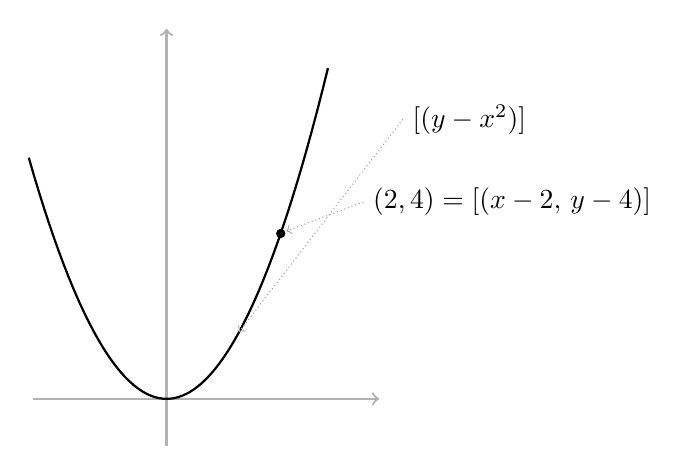
\begin{tikzpicture}[scale=1.0]
  \draw[gray!60,thick,->] (-1.7,0) -- (2.7,0);
  \draw[gray!60,thick,->] (0,-0.6) -- (0,4.7);
  \draw[thick] plot[domain=-1.75:2.05,samples=61] ({\x},{\x*\x});
  \fill (1.45,2.1) circle (1.7pt);
  \node[anchor=west] (genlab) at (3.0,3.55) {$[(y-x^2)]$};
  \draw[gray!70,densely dotted,->] (genlab.west) -- (0.92,0.85);
  \node[anchor=west] (speclab) at (2.5,2.5) {$(2,4)=[(x-2,\,y-4)]$};
  \draw[gray!70,densely dotted,->] (speclab.west) -- (1.52,2.13);
\end{tikzpicture}
\caption{$(2,4)=[(x-2,\,y-4)]$ 是 $[(y-x^2)]$ 的一个\trSpecialization{}；$[(y-x^2)]$ 是 $(2,4)$ 的一个\trGenerization{}。（依原书手绘图重绘。）}\label{fig:specialization-generization}
\end{figure}

\begin{exercise}\label{ex:specialization-primes}
设 $X=\Spec A$，证明：$[\mathfrak{q}]$ 是 $[\mathfrak{p}]$ 的一个\trSpecialization{}，当且仅当 $\mathfrak{p}\subset\mathfrak{q}$。进而证明 $V(\mathfrak{p})=\overline{\{[\mathfrak{p}]\}}$。
\end{exercise}

\textbf{3.6.11.}\ \emph{\trhDefinition{}。}\quad 设 $K$ 是一个\trClosedSubset。若 $\overline{\{p\}}=K$，就称\trTopologicalSpace{}的点 $p\in X$ 是 $K$ 的一个\textbf{\trGenericPoint}（generic point）。

这个重要概念早于\trGrothendieck{}而存在。二十世纪初的意大利代数几何学派对簇的「\trGenericPoint」已有一个概念：他们指的是不带任何特殊性质的点，于是凡对「一个\trGenericPoint」证明了的命题，对簇上「几乎所有」的点都真。现代的「\trGenericPoint」有着同样的直观含义。如果某件事对不可约子集的诸点「泛性地」或「大体地」成立——即对某个\trDense{}\trOpenSubset（对应「几乎所有的点」）成立——那么它对\trGenericPoint{}成立，反之亦然。（这是一条原理性的陈述，而非事实陈述。一个有趣的情形是「既约性」：这条原理对一般的概形并不成立，但对诸如簇这样「合理」的概形则\emph{确实}成立；参看注记~5.2.2。）例如，一个函数在不可约概形的\trGenericPoint{}处取值为零，当且仅当它在所有点处都取值为零。请留心这类其他例子。

\textbf{\trGeneralPoint{}}（general point）这个词的含义则不同。「$X$ 的\trGeneralPoint{}满足如此这般的性质」这句话，意思是「$X$ 的某个\trDense{}\trOpenSubset{}的每个点都满足如此这般的性质」。当心不要混淆「泛」与「一般」。但要警惕：公认的术语并不总遵循这条约定；「一般光滑性」（\S21.6.3）与「一般平坦性」（定理~24.5.13）便是明证。\footnote{译注：为与「一般点」（generic point，见\trGenericPoint）相区分，本译本把 general point 固定译作「\trGeneralPoint{}」。}

\begin{exercise}\label{ex:generic-point-parabola}
验证 $[(y-x^2)]\in\mathbb{A}^2_{\mathbb{C}}$ 是 $V(y-x^2)$ 的一个\trGenericPoint。
\end{exercise}

再给「一般」这个术语一点动机：我们把 $[(y-x^2)]$ 想成抛物线上某个不特定的点（而闭点 $(a,a^2)\in\mathbb{C}^2$，即 $(x-a,\,y-a^2)$（其中 $a\in\mathbb{C}$），则是「特定的点」）；按这个词的日常用法，它也是「一般的」。我们可以把它「\trSpecialization{}」到抛物线的某个特定的点；于是例如，$(2,4)$ 就是 $[(y-x^2)]$ 的一个\trSpecialization{}。（再一次，见图~\ref{fig:specialization-generization}。）为把这件事讲得更精确些：

\begin{exercise}[容易的练习]\label{ex:generic-point-near-every-point}
设 $\mathfrak{p}$ 是\trClosedSubset{} $K$ 的一个\trGenericPoint。证明它「邻近 $K$ 的每个点 $\mathfrak{q}$」（$\mathfrak{q}$ 的每个\trNeighborhood{}都含有 $\mathfrak{p}$），并且「不邻近任何不在 $K$ 中的点 $\mathfrak{r}$」（存在 $\mathfrak{r}$ 的一个不含 $\mathfrak{p}$ 的\trNeighborhood）。（这一想法曾在 \S3.2.4 例~1 与\cref{ex:topological-space-a1k} 中出现过。）
\end{exercise}

我们很快就会看到（练习~3.7.F）：$\Spec A$ 的点与 $\Spec A$ 的不可约闭子集之间有一个自然双射，它把每个点送到其闭包，把每个不可约闭子集送到它的（唯一的）\trGenericPoint。你现在就可以证明这件事，但我们想等发展出一些便利的术语再说。

\textbf{3.6.12.\ \trIrreducibleComponent{}、\trConnectedComponent{}，以及诸\trNoetherian{}条件。}\quad \trTopologicalSpace{}的一个\textbf{\trIrreducibleComponent{}}（irreducible component）是一个极大的\trIrreducible{}子集（即不被任何更大的\trIrreducible{}子集包含的\trIrreducible{}子集）。\trIrreducibleComponent{}都是闭的（因为\trIrreducible{}子集的闭包仍\trIrreducible，\cref{ex:irreducible-open-dense}(b)），而且把\trTopologicalSpace{} $X$ 的\trIrreducibleComponent{}想成 $X$ 的诸\trIrreducible{} \emph{闭}子集中的极大者，会有帮助。我们把它们看作「$X$ 的诸块」（见图~\ref{fig:irreducible-components}）。

\begin{figure}[htbp]
\centering
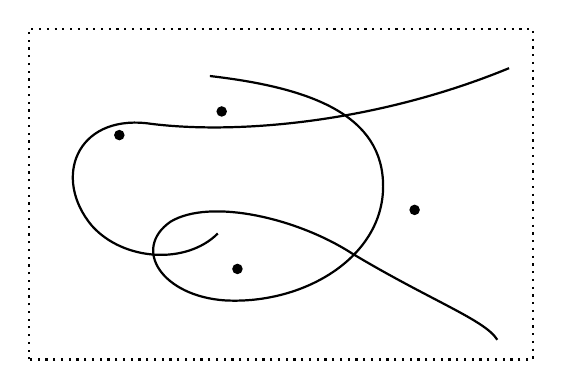
\begin{tikzpicture}[scale=1.0]
  \draw[dotted,thick] (-3.2,-2.1) rectangle (3.2,2.1);
  \draw[thick] (2.9,1.6) .. controls (1.2,0.9) and (-0.6,0.75) .. (-1.7,0.9)
    .. controls (-2.6,1.0) and (-2.9,0.2) .. (-2.4,-0.4)
    .. controls (-2.0,-0.85) and (-1.2,-0.9) .. (-0.8,-0.5);
  \draw[thick] (-0.9,1.5) .. controls (0.4,1.35) and (1.3,1.0) .. (1.3,0.1)
    .. controls (1.3,-0.8) and (0.3,-1.4) .. (-0.7,-1.35)
    .. controls (-1.5,-1.3) and (-1.9,-0.7) .. (-1.4,-0.35)
    .. controls (-0.9,-0.05) and (0.2,-0.3) .. (0.9,-0.75)
    .. controls (1.9,-1.35) and (2.6,-1.6) .. (2.75,-1.85);
  \fill (-2.05,0.75) circle (1.9pt);
  \fill (-0.75,1.05) circle (1.9pt);
  \fill (-0.55,-0.95) circle (1.9pt);
  \fill (1.7,-0.2) circle (1.9pt);
\end{tikzpicture}
\caption{$\mathbb{A}^2_{\mathbb{C}}$ 的这个\trClosedSubset{}有六个\trIrreducibleComponent{}。（依原书手绘图重绘。）}\label{fig:irreducible-components}
\end{figure}

类似地，\trTopologicalSpace{} $X$ 的子集 $Y$ 若是极大的\trConnected{}子集（即不被任何更大的\trConnected{}子集包含的\trConnected{}子集），就称为一个\textbf{\trConnectedComponent{}}（connected component）。

\begin{exercise}[每个\trTopologicalSpace{}都是诸\trIrreducibleComponent{}之并]\label{ex:point-in-irreducible-component}
证明\trTopologicalSpace{} $X$ 的每个点 $p$ 都含于 $X$ 的某个\trIrreducibleComponent{}。提示：\trZornsLemma。更精确地说，考虑由 $X$ 的含 $p$ 的诸\trIrreducible{}子集所组成的\trPoset{} $\scr S$。证明 $\scr S$ 存在极大的全序子集 $\{Z_\alpha\}$。证明 $\bigcup Z_\alpha$ 是\trIrreducible{}的。
\end{exercise}

\textbf{3.6.13.}\ \emph{\trhRemark{}。}\quad 每个点都含于某个\trConnectedComponent{}，而\trConnectedComponent{}总是闭的。你现在就可以证明这件事，但我们刻意把它推迟到需要它之时，那是一个带星的选学小节（练习~10.5.J）。另一方面，\trConnectedComponent{}未必是开的；参看 [Stacks, tag 004T]。\trConnectedComponent{}不是开集的\trAffineScheme{}的一个例子是 $\Spec\bigl(\prod_i^{\infty}\mathbb{F}_2\bigr)$。

\textbf{3.6.14.}\quad 在我们考虑过的诸例中，这些空间都自然地分裂成有限多个\trIrreducibleComponent{}。例如，$\mathbb{A}^2_k$ 中 $xy=0$ 的\trLocus，我们把它想成有两「块」——两条坐标轴。原因在于：它们的底\trTopologicalSpace（我们很快将予确立）是\textbf{\trNoetherian}（Noetherian）的。若\trTopologicalSpace{} $X$ 对\trClosedSubset{}满足\textbf{\trDescendingChainCondition{}}（descending chain condition）：任何一列\trClosedSubset{} $Z_1\supset Z_2\supset\cdots\supset Z_n\supset\cdots$ 都终将稳定下来——存在 $r$ 使得 $Z_r=Z_{r+1}=\cdots$——就称 $X$ 是\trNoetherian{}的。这里给出第一个例子（你应当不用\trNoetherian{}环而把它显式做出来）。

\begin{exercise}\label{ex:a2-noetherian}
证明 $\mathbb{A}^2_{\mathbb{C}}$ 是\trNoetherian{}\trTopologicalSpace：$\mathbb{A}^2_{\mathbb{C}}=\Spec\mathbb{C}[x,y]$ 的任何一列递减的\trClosedSubset{}都必终将稳定。注意稳定所需的时长可以任意长。（$\mathbb{A}^2_{\mathbb{C}}$ 的诸\trClosedSubset{}已在 \S3.4.5 中描述过。）证明：带\trClassicalTopology{}的 $\mathbb{C}^2$ \emph{不是}\trNoetherian{}\trTopologicalSpace。
\end{exercise}

\textbf{3.6.15.}\ \textbf{\trhProposition{}。}\ ——\ \emph{设 $X$ 是\trNoetherian{}\trTopologicalSpace。则每个非空\trClosedSubset{} $Z$ 都能唯一地表示成有限并 $Z=Z_1\cup\cdots\cup Z_n$，其中诸 $Z_i$ 是\trIrreducible{}的\trClosedSubset，且没有一个包含于另一个之中。}

翻译一下：任何\trClosedSubset{} $Z$ 都只有有限多个「块」。

\emph{证明。}\quad 下述技术称为\textbf{诺特归纳}（Noetherian induction），理由将会明朗。我们还会多次使用它。考虑 $X$ 的那些\emph{不能}表示成不可约闭子集之有限并的非空\trClosedSubset{}所成的族。我们来证明这个族是空的。否则，设 $Y_1$ 是其中一个。若 $Y_1$ 真包含另一个这样的成员，就选一个，称为 $Y_2$。若 $Y_2$ 又真包含另一个这样的成员，就选一个，称为 $Y_3$，如此等等。由\trDescendingChainCondition{}，这个过程必终将停止，于是我们有某个 $Y_r$，它不能写成不可约闭子集的有限并，但真包含于它的每个\trClosedSubset{}却都能这样写。然而 $Y_r$ 自身并不可约，故可写 $Y_r=Y'\cup Y''$，其中 $Y'$ 与 $Y''$ 都是真\trClosedSubset。由假设，这两者都能写成有限多个不可约闭子集之并，于是 $Y_r$ 也能，矛盾。这样一来，每个\trClosedSubset{}都能写成不可约闭子集的有限并。通过丢弃其中若干个，不妨设这些不可约闭子集互不包含。

我们接着证唯一性。设
\[
Z=Z_1\cup Z_2\cup\cdots\cup Z_r=Z'_1\cup Z'_2\cup\cdots\cup Z'_s
\]
是两种这样的表示。则 $Z'_1\subset Z_1\cup Z_2\cup\cdots\cup Z_r$，于是 $Z'_1=(Z_1\cap Z'_1)\cup\cdots\cup(Z_r\cap Z'_1)$。现在 $Z'_1$ 是\trIrreducible{}的，故这些成员之一就是 $Z'_1$ 本身，比如说（不失一般性）$Z_1\cap Z'_1$。于是 $Z'_1\subset Z_1$。类似地，$Z_1\subset Z'_\alpha$ 对某个 $\alpha$ 成立；但由于 $Z'_1\subset Z_1\subset Z'_\alpha$，而 $Z'_1$ 不含于其他任何 $Z'_j$，必有 $\alpha=1$，从而 $Z'_1=Z_1$。这样，$Z$-名单中的每个成员都在 $Z'$-名单中，反之亦然，所以两张名单必是同一张。\hfill$\square$

\begin{exercise}\label{ex:connected-components-union-irreducible}
证明\trTopologicalSpace{} $X$ 的每个\trConnectedComponent{}都是 $X$ 的若干\trIrreducibleComponent{}之并。证明：$X$ 的任何同时开且闭的子集必是 $X$ 的某几个\trConnectedComponent{}之并。设 $X$ 是\emph{\trNoetherian}的\trTopologicalSpace，证明：$X$ 的任意一组\trConnectedComponent{}之并总是在 $X$ 中既开又闭。（特别地，\trNoetherian{}\trTopologicalSpace{}的\trConnectedComponent{}总是开的；这对更一般的\trTopologicalSpace{}并不成立，参看注记~3.6.13。）
\end{exercise}

\textbf{3.6.16.\ \trNoether{}环。}\quad 事实证明，我们考虑过的全部谱（带星的\cref{ex:spec-quasicompact}(b) 除外）都是\trNoetherian{}\trTopologicalSpace，但这并非对一切环的谱都成立。我们的例子所共有的关键特征是：这些环都是\emph{\trNoetherian}的。若一个\trRing{}的诸\trIdeal{}的每个升链 $I_1\subset I_2\subset\cdots$ 都终将稳定：存在 $r$ 使得 $I_r=I_{r+1}=\cdots$，就称它是\textbf{\trNoetherian}的。（这对\trIdeal{}而言称为\textbf{\trAscendingChainCondition{}}（ascending chain condition）。）

下面是关于\trNoetherian{}环的几条速记事实。你应当能把它们全部证明：
\begin{itemize}
\item \trField{}都是\trNoetherian{}的。$\mathbb{Z}$ 是\trNoetherian{}的。
\item （\trNoetherian{}性在取商下保持。）若 $A$ 是\trNoetherian{}的，$I$ 是 $A$ 的任一\trIdeal，则 $A/I$ 是\trNoetherian{}的。
\item （\trNoetherian{}性在\trLocalization{}下保持。）若 $A$ 是\trNoetherian{}的，$S$ 是任一\trMultiplicativeSubset，则 $S^{-1}A$ 是\trNoetherian{}的。
\end{itemize}

\begin{exercise}\label{ex:pid-noetherian}
证明\trPID{}都是\trNoetherian{}环。
\end{exercise}

\begin{exercise}[重要练习]\label{ex:noetherian-finitely-generated-ideals}
证明：\trRing{} $A$ 是\trNoetherian{}的，当且仅当 $A$ 的每个\trIdeal{}都是\trFinitelyGenerated{}的。
\end{exercise}

下一条事实就不平凡了。

\textbf{3.6.17.\ \trHilbert{}基定理。}\ ——\ \emph{若 $A$ 是\trNoetherian{}的，则 $A[x]$ 亦然。}

\trHilbert{}在划时代的论文 [Hil] 中证明了这个定理；他还在同一篇论文中证明了\trHilbert{}合冲定理（\S16.1.2），并定义了\trHilbert{}函数，证明它们最终成为多项式（\S18.6）。

\textbf{3.6.18.}\quad 由上述结果，任意域上的、或者整数环上的有限多元多项式环都是\trNoetherian{}的——其任何商或局部化亦然。于是例如，$k$ 或 $\mathbb{Z}$ 上任何有限生成的代数，以及其任何局部化，都是\trNoetherian{}的。大多数「好」环都是\trNoetherian{}的，但并非所有的环都\trNoetherian：$k[x_1,x_2,\dots]$ 就不是，因为 $(x_1)\subset(x_1,x_2)\subset(x_1,x_2,x_3)\subset\cdots$ 是\trIdeal{}的一条严格升链（参看\cref{ex:spec-quasicompact}(b)）。

\textbf{3.6.19.}\ \emph{\trHilbert{}基定理 3.6.17 的证明。}\quad 我们来证明\trIdeal{} $I\subset A[x]$ 都是\trFinitelyGenerated{}的。我们归纳地构造一组生成元 $f_1,\dots$，方法如下。对 $n\ge 0$，若 $I\neq(f_1,\dots,f_n)$，就取 $f_{n+1}$ 为 $I-(f_1,\dots,f_n)$ 中次数最低的任一非零元素。于是（假定 $I\neq(0)$）$f_1$ 就是 $I$ 中次数最低的任一元素。若这个程序终止，我们就完成了。否则，令 $a_n\in A$ 为 $f_n$ 的最低次项系数（对一切 $n>0$）。由于 $A$ 是\trNoetherian{}的，存在 $N$ 使得 $(a_1,a_2,\dots)=(a_1,\dots,a_N)$。设 $a_{N+1}=\sum_{i=1}^{N}b_ia_i$。那么
\[
f_{N+1}-\sum_{i=1}^{N}b_if_ix^{\deg f_{N+1}-\deg f_i}
\]
是 $I$ 中一个不属于 $(f_1,\dots,f_N)$ 的元素（因为 $f_{N+1}\notin(f_1,\dots,f_N)$），并且次数低于 $f_{N+1}$，这与我们本应选取 $f_{N+1}$ 的方式相矛盾。\hfill$\square$

现在我们把\trNoetherian{}环与\trNoetherian{}\trTopologicalSpace{}联系起来。

\begin{exercise}\label{ex:noetherian-ring-spec-noetherian}
设 $A$ 是\trNoetherian{}的，证明 $\Spec A$ 是\trNoetherian{}\trTopologicalSpace。描述一个\trRing{} $A$，使得 $\Spec A$ 不是\trNoetherian{}\trTopologicalSpace。（题外话：若 $\Spec A$ 是\trNoetherian{}\trTopologicalSpace，$A$ 未必\trNoetherian。一个例子是 $A=k[x_1,x_2,x_3,\dots]/(x_1,\,x_2^2,\,x_3^3,\dots)$。此时 $\Spec A$ 只有一个点，因而是\trNoetherian{}的。但 $A$ 不是\trNoetherian{}的，因为在 $A$ 中 $(x_1)\subsetneq(x_1,x_2)\subsetneq(x_1,x_2,x_3)\subsetneq\cdots$。）
\end{exercise}

\begin{exercise}[练习~3.6.G(b) 所许诺的]\label{ex:noetherian-open-quasicompact}
证明\trNoetherian{}\trTopologicalSpace{}的每个\trOpenSubset{}都是\trQuasicompact{}的。于是若 $A$ 是\trNoetherian{}的，$\Spec A$ 的每个\trOpenSubset{}都是\trQuasicompact{}的。（如果你愿意，也可以对带诱导拓扑的\emph{任何}子集证明这个结果。）
\end{exercise}

\textbf{3.6.20.\ 留供后用：模的\trNoetherian{}条件。}\quad 一个重要的相关概念是\trNoetherian{}\emph{模}。虽然我们要过一阵子才会用到这个概念（\S10.7.3），但我们打算趁\trNoetherian{}观念在你脑海中还新鲜之时，发展其最重要的性质。设 $A$ 是任一\trRing，不必\trNoetherian。若一个 $A$-模对子模满足\trAscendingChainCondition{}，就称这个 $A$-模是\textbf{\trNoetherian}的（Noetherian $A$-module）。于是例如：\trRing{} $A$ 是\trNoetherian{}的，当且仅当它作为 $A$-模是\trNoetherian{}的。

\begin{exercise}[参看重要的\cref{ex:noetherian-finitely-generated-ideals}]\label{ex:noetherian-module-submodule-fg}
证明：若 $M$ 是\trNoetherian{} $A$-模，则 $M$ 的任何子模都是\trFinitelyGenerated{}的 $A$-模。（事实上逆命题也真，你尽管把它也证了。）
\end{exercise}

\begin{exercise}\label{ex:noetherian-module-extension}
若 $0\to M'\to M\to M''\to 0$ 是\trExactSequence，证明：$M'$ 与 $M''$ 是\trNoetherian{}的，当且仅当 $M$ 是\trNoetherian{}的。（提示：给定 $M$ 中的一条升链，我们在 $M'$ 与 $M''$ 中得到两条同步的升链。可能的进一步提示：证明：若
\[
M'\longrightarrow M\xrightarrow{\ \phi\ }M''
\]
是\trExactSequence，$N\subset N'\subset M$，且 $N\cap M'=N'\cap M'$、$\phi(N)=\phi(N')$，则 $N=N'$。）
\end{exercise}

\begin{exercise}\label{ex:noetherian-free-module}
证明：若 $A$ 是\trNoetherian{}环，则 $A^{\oplus n}$ 是\trNoetherian{} $A$-模。
\end{exercise}

\begin{exercise}\label{ex:finitely-generated-noetherian-module}
证明：若 $A$ 是\trNoetherian{}环，$M$ 是有限生成的 $A$-模，则 $M$ 是\trNoetherian{}模。于是由\cref{ex:noetherian-module-submodule-fg}：\trNoetherian{}环上有限生成模的任何子模都是有限生成的。
\end{exercise}

\textbf{3.6.21.\ 你为什么不必为\trNoetherian{}假设操心。}\quad 你该不该辛辛苦苦去消除\trNoetherian{}假设？你该不该为\trNoetherian{}假设操心？你该不该夜里睡不着觉、满脑子想着非\trNoetherian{}环？对大多数人来说，这些问题的答案是「不必」。多数人永远不需要为非\trNoetherian{}环操心，但也有理由对它们持开放态度。首先，它们真的会冒出来。例如，\trNoetherian{}\trScheme{}在\trNoetherian{}\trScheme{}上的\trFiberProduct（甚至连\trNoetherian{}点在\trNoetherian{}点上的\trFiberProduct！）可以是非\trNoetherian{}的（警告~10.1.5），而\trNoetherian{}环的\trNormalization{}也可以是非\trNoetherian{}的（警告~10.7.4）。你可以辛苦地去证明你关心的那些环或概形没有这种病态，也可以索性放松，不去操心它。其次，一般地与概形打交道往往并无害处。知道何时需要\trNoetherian{}条件，会帮你记住结果为何为真，因为你会对\trNoetherian{}条件从何处进入论证有某种感觉。最后，对某些人来说，非\trNoetherian{}环会自然出现。例如，阿代尔（ad\`ele）不是\trNoetherian{}的。而算术与热带几何中自然出现的许多\trValuationRing{}（valuation ring）也都不是\trNoetherian{}的。


\section{函数 $I(\cdot)$：从 $\Spec A$ 的子集到理想}

现在，我们引入一个概念，它在某种意义上是\trVanishingSet{}函数 $V(\cdot)$ 的
「逆」。给定 $\Spec A$ 的一个子集 $S$，$I(S)$ 是在 $S$ 上消失的那些函数所成的
集合；换言之，$I(S)=\bigcap_{[\mathfrak{p}]\in S}\mathfrak{p}\subset A$
（至少当 $S$ 非空时是如此）。

我们快速地作三条观察。（你能看出它们为什么都成立吗？）
\begin{itemize}
\item $I(S)$ 显然是 $A$ 的一个\trIdeal。
\item $I(\cdot)$ 反转包含关系：若 $S_1\subset S_2$，则 $I(S_2)\subset I(S_1)$。
\item $I(\overline{S})=I(S)$。
\end{itemize}

\begin{exercise}\label{ex:i-of-axis-and-point}
设 $A=k[x,y]$。若 $S=\{[(y)],\,[(x,y-1)]\}$（见图~\ref{fig:set-of-37a}），则
$I(S)$ 由那些在 $x$-轴上消失、并且在点 $(0,1)$ 处消失的多项式组成。试给出这个\trIdeal{}的生成元。
\end{exercise}

\begin{exercise}\label{ex:i-of-three-axes}
设 $S\subset\mathbb{A}^3_{\mathbb{C}}$ 是三条坐标轴的并。给出\trIdeal{} $I(S)$ 的生成元。务必给出证明！我们将在练习~13.1.F 中看到，这个\trIdeal{}无法由少于三个元素生成。
\end{exercise}

\begin{figure}[htbp]
\centering
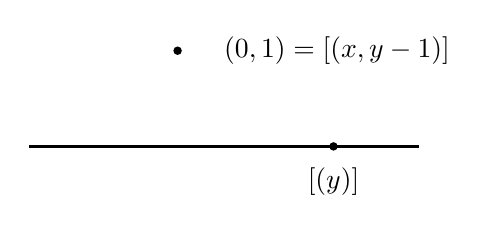
\begin{tikzpicture}[scale=0.9]
  \draw[thick] (-2.4,0) -- (3.1,0);
  \fill (1.9,0) circle (1.7pt) node[below=4pt] {$[(y)]$};
  \fill (-0.3,1.35) circle (1.7pt);
  \node at (1.95,1.35) {$(0,1)=[(x,y-1)]$};
\end{tikzpicture}
\caption{\cref{ex:i-of-axis-and-point} 的集合 $S$，画作 $\mathbb{A}^2$ 的一个子集。（依原书手绘图重绘。）}\label{fig:set-of-37a}
\end{figure}

\begin{exercise}\label{ex:v-of-i-is-closure}
证明 $V(I(S))=\overline{S}$。于是，当 $S$ 是\trClosedSet{}时，$V(I(S))=S$。
\end{exercise}

注意，$I(S)$ 总是一个\trRadicalIdeal——若 $f\in\sqrt{I(S)}$，则对某个 $n>0$，
$f^n$ 在 $S$ 上消失；于是 $f$ 在 $S$ 上消失，从而 $f\in I(S)$。

\begin{exercise}[容易的练习]\label{ex:i-of-v-is-radical}
证明：若 $J\subset A$ 是一个\trIdeal，则 $I(V(J))=\sqrt{J}$。（巨大的提示：\cref{ex:vanish-on-vi-radical}。）
\end{exercise}

\cref{ex:v-of-i-is-closure} 与 \cref{ex:i-of-v-is-radical} 表明，$V$ 与 $I$
是「差不多」互逆的。更精确地说：

\begin{theorem}\label{thm:closed-subsets-radical-ideals}
$V(\cdot)$ 与 $I(\cdot)$ 在 $\Spec A$ 的诸\trClosedSubset{}与 $A$ 的诸\trRadicalIdeal{}之间给出一个反转包含关系的双射（其中\trClosedSubset{}经 $I(\cdot)$ 给出\trRadicalIdeal，而\trRadicalIdeal{}经 $V(\cdot)$ 给出\trClosedSubset）。
\end{theorem}

\cref{thm:closed-subsets-radical-ideals} 有时被称为\trHilbert{}\trNullstellensatz，但我们把这个名字保留给 \cref{thm:hilbert-nullstellensatz}。

\begin{exercise}\label{ex:i-of-v-exceeds-j}
设 $J=(x^2+y^2-1,\,y-1)$。找出 $I(V(J))\smallsetminus J$ 中的一个元素，并给出证明。
\end{exercise}

\begin{exercise}[重要练习；参看\cref{ex:minimal-prime-ideals}]\label{ex:irreducible-prime-bijection}
证明：$V(\cdot)$ 与 $I(\cdot)$ 给出 $\Spec A$ 的\emph{\trIrreducible{}\trClosedSubset}与 $A$ 的\emph{\trPrimeIdeal}之间的一个双射。由此推证：$\Spec A$ 的点与 $\Spec A$ 的\trIrreducible{}\trClosedSubset{}之间存在双射（其中，一个点经取\trClosure{}确定一个\trIrreducible{}\trClosedSubset）。于是，\emph{$\Spec A$ 的每个\trIrreducible{}\trClosedSubset{}都恰有一个\trGenericPoint}——任何\trIrreducible{}\trClosedSubset{} $Z$ 都能唯一地写成 $\overline{\{z\}}$。
\end{exercise}

\begin{exercise}[练习兼定义]\label{ex:minimal-prime-ideals}
环 $A$ 的一个\trPrimeIdeal{}称为\textbf{\trMinimalPrimeIdeal{}}（minimal prime ideal）
（或者更简单些，\textbf{\trMinimalPrime{}}（minimal prime）），如果它在包含关系之下是极小的。（例如，$k[x,y]$ 的唯一\trMinimalPrimeIdeal{}是 $(0)$。）设 $A$ 是任意的环，证明 $\Spec A$ 的\trIrreducibleComponent{}与 $A$ 的\trMinimalPrimeIdeal{}之间存在双射。特别地，$\Spec A$ 是\trIrreducible{}的，当且仅当 $A$ 只有一个\trMinimalPrimeIdeal{}；这推广了\cref{ex:integral-domain-irreducible}。
\end{exercise}

命题~3.6.15、\cref{ex:noetherian-ring-spec-noetherian} 与 \cref{ex:minimal-prime-ideals} 蕴含：每个\trNoether{}环都只有有限多个\trMinimalPrimeIdeal{}。一个代数事实，如今被揭示出来：它其实是一个「几何」事实！

\begin{exercise}[现实检验]\label{ex:irreducible-factors-components}
在 $\mathbb{A}^n_k=\Spec k[x_1,\dots,x_n]$ 中，由 $f(x_1,\dots,x_n)\in k[x_1,\dots,x_n]$ 切出的子集，理应具有一些\trIrreducibleComponent{}，与 $f$ 的互不相同的\trIrreducible{}因子相对应。证明这一点。（环 $k[x_1,\dots,x_n]$ 的什么性质使这件事得以成立？）
\end{exercise}

\begin{exercise}\label{ex:minimal-primes-quotient-xy}
$k[x,y]/(xy)$ 的\trMinimalPrimeIdeal{}是什么（其中 $k$ 是一个\trField）？
\end{exercise}

\textbf{3.7.2.\ 代数与几何之间一部宏大词典的开端。}\quad 我们此刻已在编纂一部代数与几何之间的宏大词典的路上行进了很远；随着理解的日益加深，你应当不断为这张表增补词条。

\begin{table}[htbp]
  \centering
  \footnotesize
  \begin{tabular}{|>{\raggedright\arraybackslash}p{5.6cm}|>{\raggedright\arraybackslash}p{5.2cm}|>{\raggedright\arraybackslash}p{2.6cm}|}
    \hline
    代数 & 几何 & 参看 \\
    \hline
    \trRing{} $A$ & \trAffineScheme{} $\Spec A$ & \mbox{\S3.2.1} \\
    \hline
    $\mathfrak{p}=I(\mathfrak{p})$：$A$ 的\trPrimeIdeal & $\mathfrak{p}=[\mathfrak{p}]$：$\Spec A$ 的点 & \mbox{\S3.2.1}、\mbox{\S3.7} \\
    \hline
    元素 $f\in A$ & $\Spec A$ 上的函数 $f$ & \mbox{\S3.2.1} \\
    \hline
    $f\pmod{\mathfrak{p}}$ & $f(\mathfrak{p})$；函数 $f$ 在 $\mathfrak{p}$ 处的值 & \mbox{\S3.2.1} \\
    \hline
    $f\in\mathfrak{p}$ & 函数 $f$ 在 $\mathfrak{p}$ 处消失（为零） & \mbox{\S3.2.1} \\
    \hline
    $A$ 的\trNilradical{}理想 $\mathfrak{N}=\sqrt{(0)}=\bigcap\mathfrak{p}$ & 在每一点处都消失的函数 & \mbox{\cref{thm:nilradical-intersection-primes}} \\
    \hline
    $A$ 的\trMaximalIdeal & $\Spec A$ 的作为点的\trIrreducible{}\trClosedSubset{}（即 $\Spec A$ 的\trClosedPoint） & \mbox{练习~3.6.I} \\
    \hline
    $\mathfrak{p}=I(Z)$：$A$ 的\trPrimeIdeal（又一次！） & $\Spec A$ 的\trIrreducible{}\trClosedSubset{} $Z=V(\mathfrak{p})$ & \mbox{\cref{ex:irreducible-prime-bijection}} \\
    \hline
    $A$ 的\trMinimalPrimeIdeal{} & $\Spec A$ 的\trIrreducibleComponent{} & \mbox{\cref{ex:minimal-prime-ideals}} \\
    \hline
    $A$ 的\trRadicalIdeal{} $I=\sqrt{I}=I(S)$ & $\Spec A$ 的\trClosedSubset{} $S=V(I)$ & \mbox{\cref{thm:closed-subsets-radical-ideals}} \\
    \hline
  \end{tabular}
\end{table}

